\chapter{Methodology}\label{meth}

\section{Data Specification}

All data in this study comes from StatsBomb's open data \cite{Statsbomb}, which is published free of charge as JSON files. Three kinds of file were used:
\begin{itemize}
    \item Competition Data: the competitions and seasons that are available
    \item Match Data: the matches of each competition and season, with teams and scores
    \item Event Data: every on-ball event of each match (passes, dribbles, tackles, shots and so on), and for each shot a \textit{freeze frame} giving the position of every visible player at the moment of the shot
\end{itemize}

\begin{figure}[!h]
    \centering
    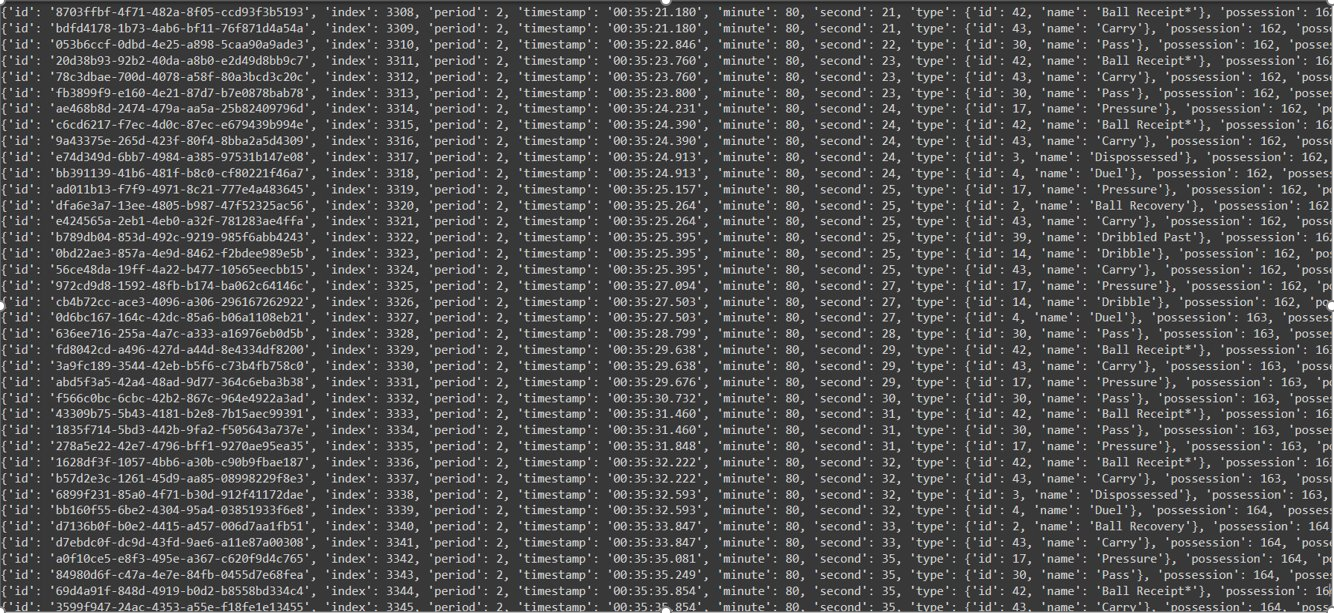
\includegraphics[scale=0.45]{images/data.png}
    \caption{Event Data Format}
    \label{data}
\end{figure}

A visual of the event data is shown in figure \ref{data}, where each row is one event of a 90 minute football match.

\subsection{Scope of the Revised Edition}

The original edition of this study used the 520 La Liga matches available in the open data at the time, all of which involved FC Barcelona. A model trained on one exceptional team learns that team's chances rather than football's, so this edition uses every men's match in the open data instead. Women's football is left out, so that the model describes one population of players.

The men's open data contains 2,651 matches and 66,854 shots, from La Liga, the Premier League, Serie A, Ligue 1, the 1. Bundesliga, the Indian Super League, the FIFA World Cup, the UEFA Euro, the Copa América, the African Cup of Nations, the Champions League and a few smaller competitions. Four of these are complete seasons: the 2015/16 Premier League, La Liga, Serie A and Ligue 1 (Ligue 1 is missing 3 of its 380 matches). The other competitions cover selected matches, such as one club's matches or a tournament.

The \textbf{modelling set} is every open-play shot from men's matches played since 2000, taken with the foot or the head: \textbf{61,003 shots and 6,277 goals (10.3\%) from 2,616 matches}. The 35 matches before 2000 were left out, because StatsBomb collected them from historical footage. Every open-play shot has a freeze frame, and 99.9\% of the freeze frames include the goalkeeper, so all the features below can be computed for the whole set.

The workflow used to develop the Expected Goals (xG) model has the following stages:
\begin{itemize}
    \item Data Cleaning/Wrangling
    \item Exploratory Data Analysis
    \item Feature Engineering
    \item Model Tuning and Evaluation
\end{itemize}

To visualise a football pitch, StatsBomb's coordinate system was followed. The pitch is 120 by 80 yards; the attacking goal is at $x = 120$, and its posts are at $y = 36$ and $y = 44$ (figure \ref{pitchspec}).

\begin{figure}[!h]
    \centering
    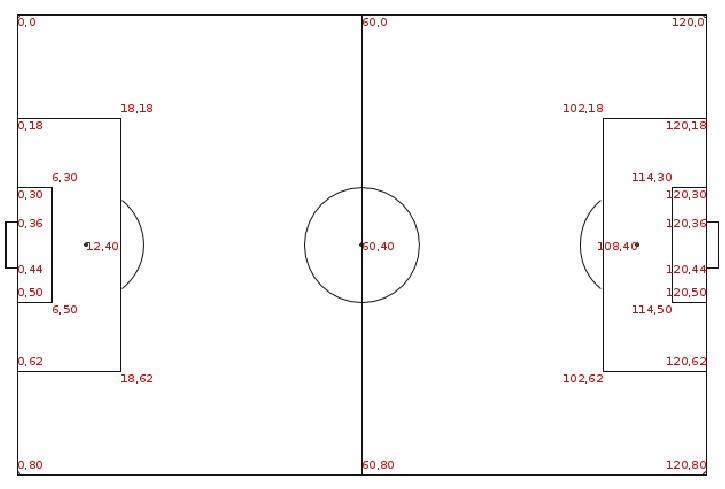
\includegraphics[scale=0.65]{images/pitchspec.jpg}
    \caption{Pitch Visualisation Specification}
    \label{pitchspec}
\end{figure}

\newpage

\section{Data Wrangling/Cleaning}

Data Wrangling is the process of turning raw data into a structured form that can be analysed. The events of every match were downloaded once and cached, and one row per shot was extracted with the following fields:

\begin{figure}[!h]
    \centering
    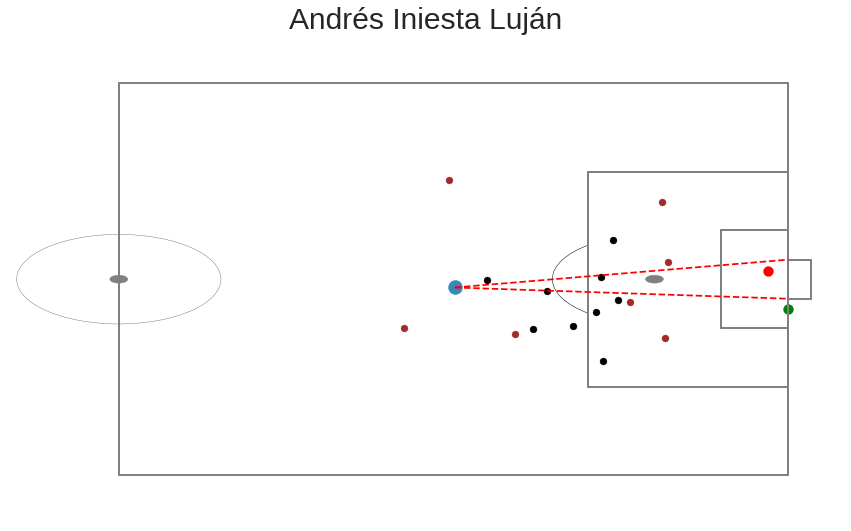
\includegraphics[scale=0.45]{images/angle.png}
    \caption{Football Pitch Visualisation}
    \label{example}
\end{figure}

\begin{itemize}
    \item Shot Id: ID of the Shot Event
    \item Play Pattern: Play Pattern preceding the Shot
    \item X Location Shot and Y Location Shot: Coordinates of the Shot
    \item Outcome: Outcome of the Shot
    \item Technique Used: The technique used to shoot the ball
    \item First Time: Whether the ball was shot with the first touch
    \item X GK Location and Y GK Location: Coordinates of the opposing Goalkeeper, from the freeze frame
    \item Body Part: The body part used
    \item Type of Shot: Open Play, Free Kick or Penalty
    \item Player Name and Team Name
    \item Official xG: xG provided by StatsBomb, kept only as a reference
    \item Pass Type: The height of the key pass before the shot (ground, low or high), or none
\end{itemize}

Two corrections were made compared with the original edition. First, the goalkeeper's position is now reset for every shot; previously, a shot whose freeze frame did not show the goalkeeper silently reused the position from the previous shot. Second, team names are taken from each match's line-ups, so that every shot is assigned to the right team. Further features were engineered from these fields, as covered in section \ref{feature}.

\newpage

\section{Exploratory Data Analysis}\label{EDA}

\begin{figure}[!h]
    \centering
    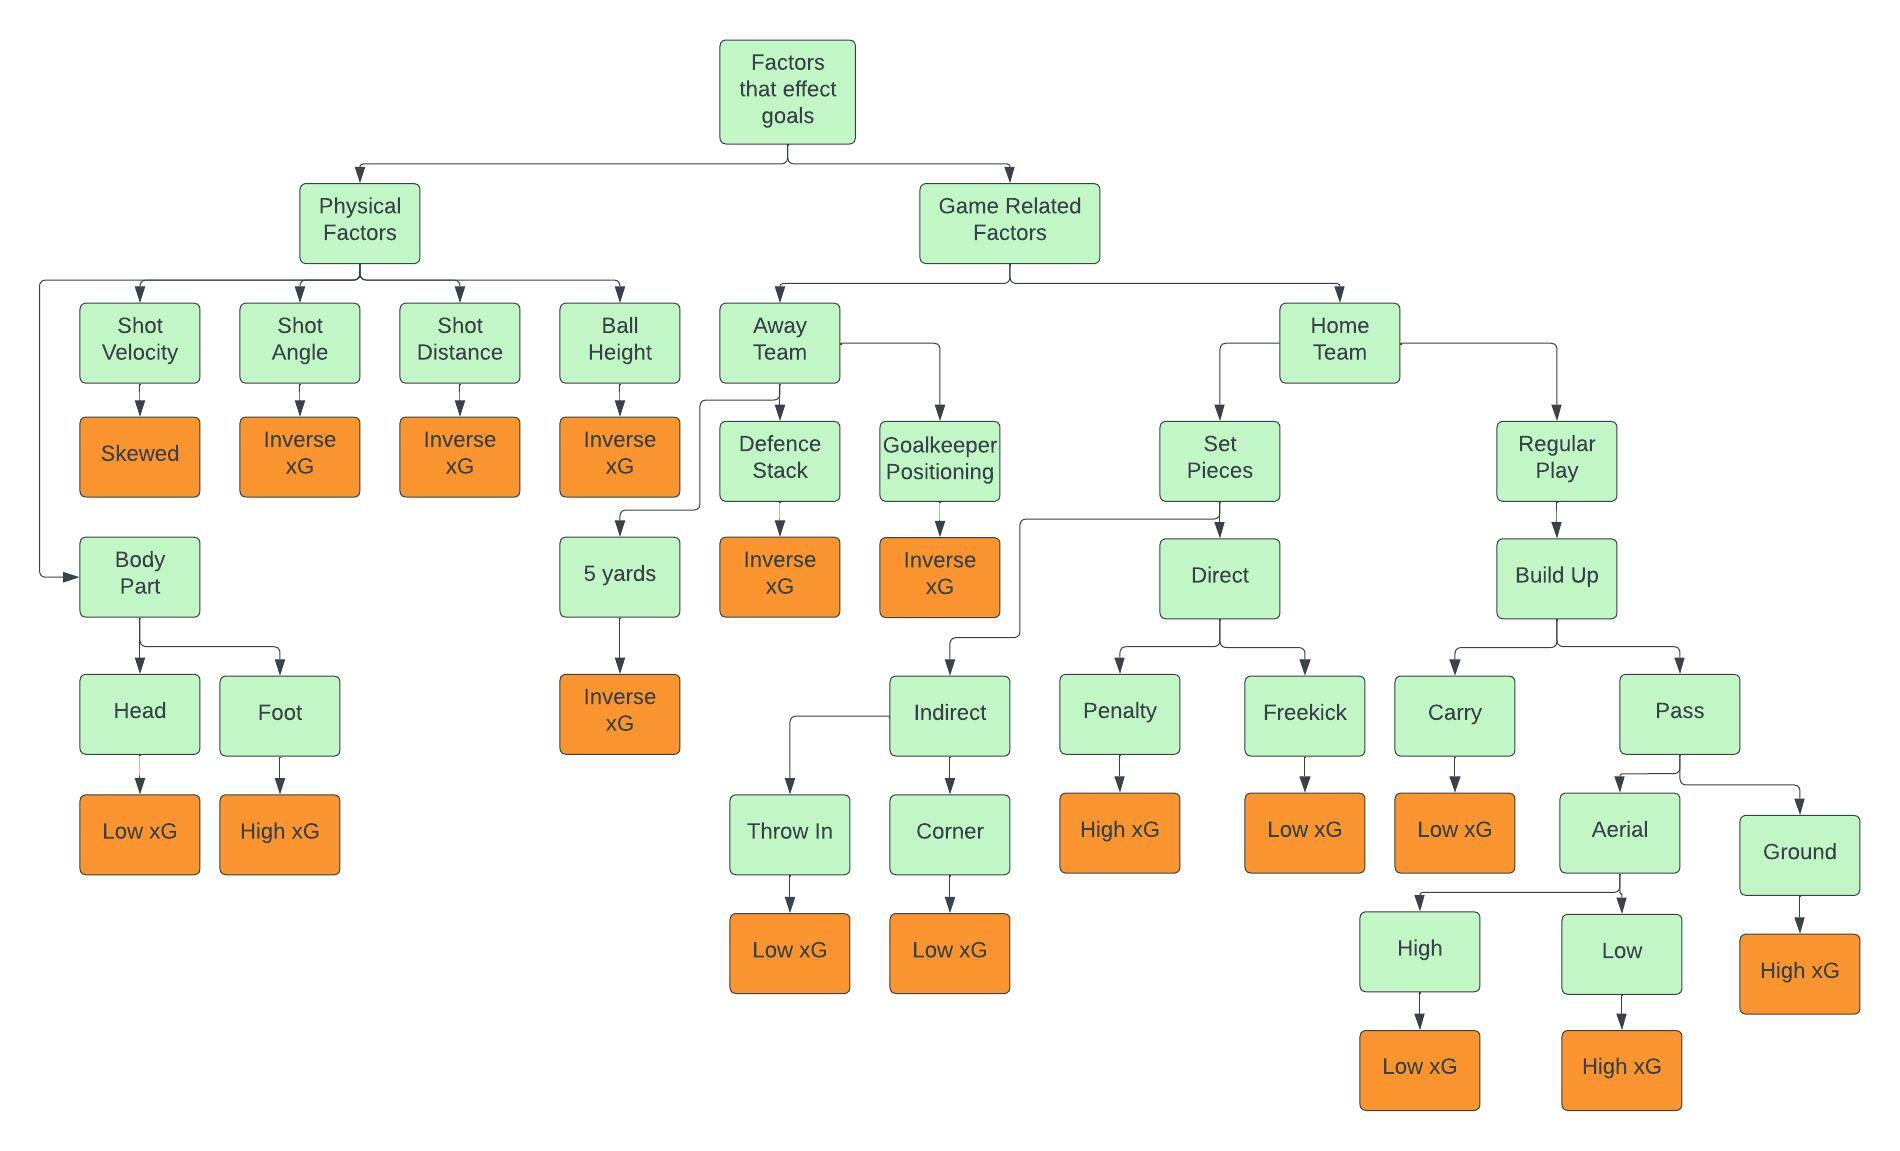
\includegraphics[scale=0.55]{images/hypothesis.jpeg}
    \caption{Hypothesis}
    \label{hypo}
\end{figure}

After the data was wrangled, it was explored to find which features matter for Machine Learning. An initial hypothesis directed this analysis and gave a road map for it (figure \ref{hypo}).

To keep the test of the models honest, the exploratory analysis uses only the \textbf{training matches}: 48,994 open-play shots and 5,024 goals (10.3\%) from 2,092 matches. The 524 matches held out for testing (section \ref{test}) were not looked at.

Many features in football are linked to shot distance: a shot close to goal is usually also taken under more pressure, at a wider angle, and more often with the head. A feature can therefore look important, or unimportant, only because of distance. Where this matters, the goal rate is compared \textbf{within bands of shot distance} as well as overall.

Each feature is analysed in turn, starting with Shot Distance.

\newpage

\subsection{Shot Distance}

Shot distance is the distance from the shot location to the centre of the goal. The hypothesis was that the chance of scoring falls with distance, and the data confirms it (figures \ref{shot distance} and \ref{histo}). More than half of all shots from within 5 yards were goals (56.4\%), against 22.3\% from 5--10 yards, 9.9\% from 15--20 yards and under 2.5\% from beyond 25 yards.

\begin{figure}[!h]
    \centering
    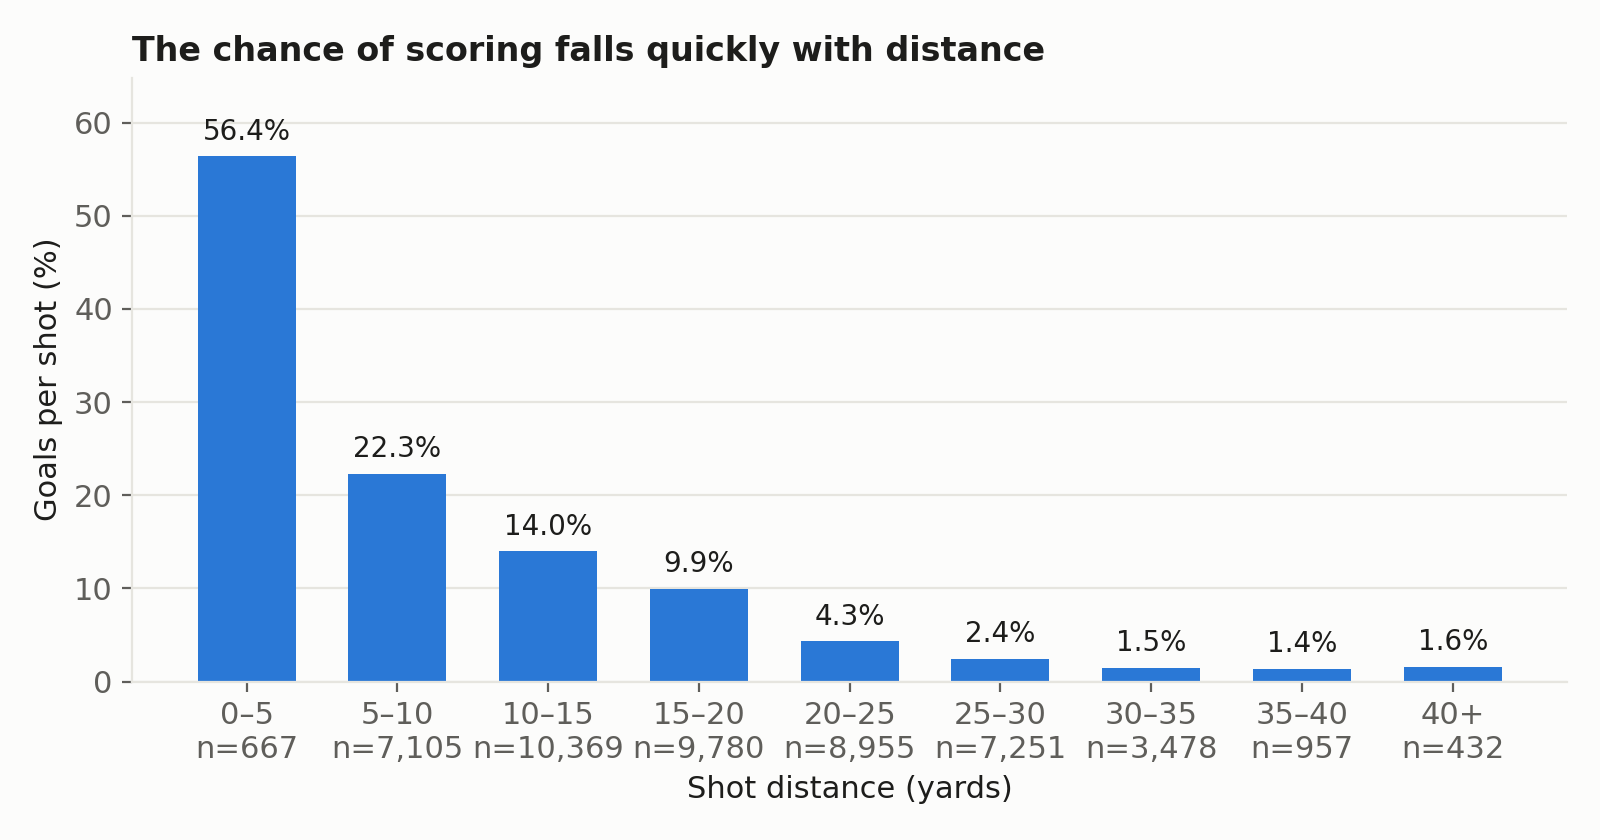
\includegraphics[width=0.9\textwidth]{images/shot distance.png}
    \caption{Goal Percentage in 5 yard Intervals}
    \label{shot distance}
\end{figure}

\begin{figure}[!h]
    \centering
    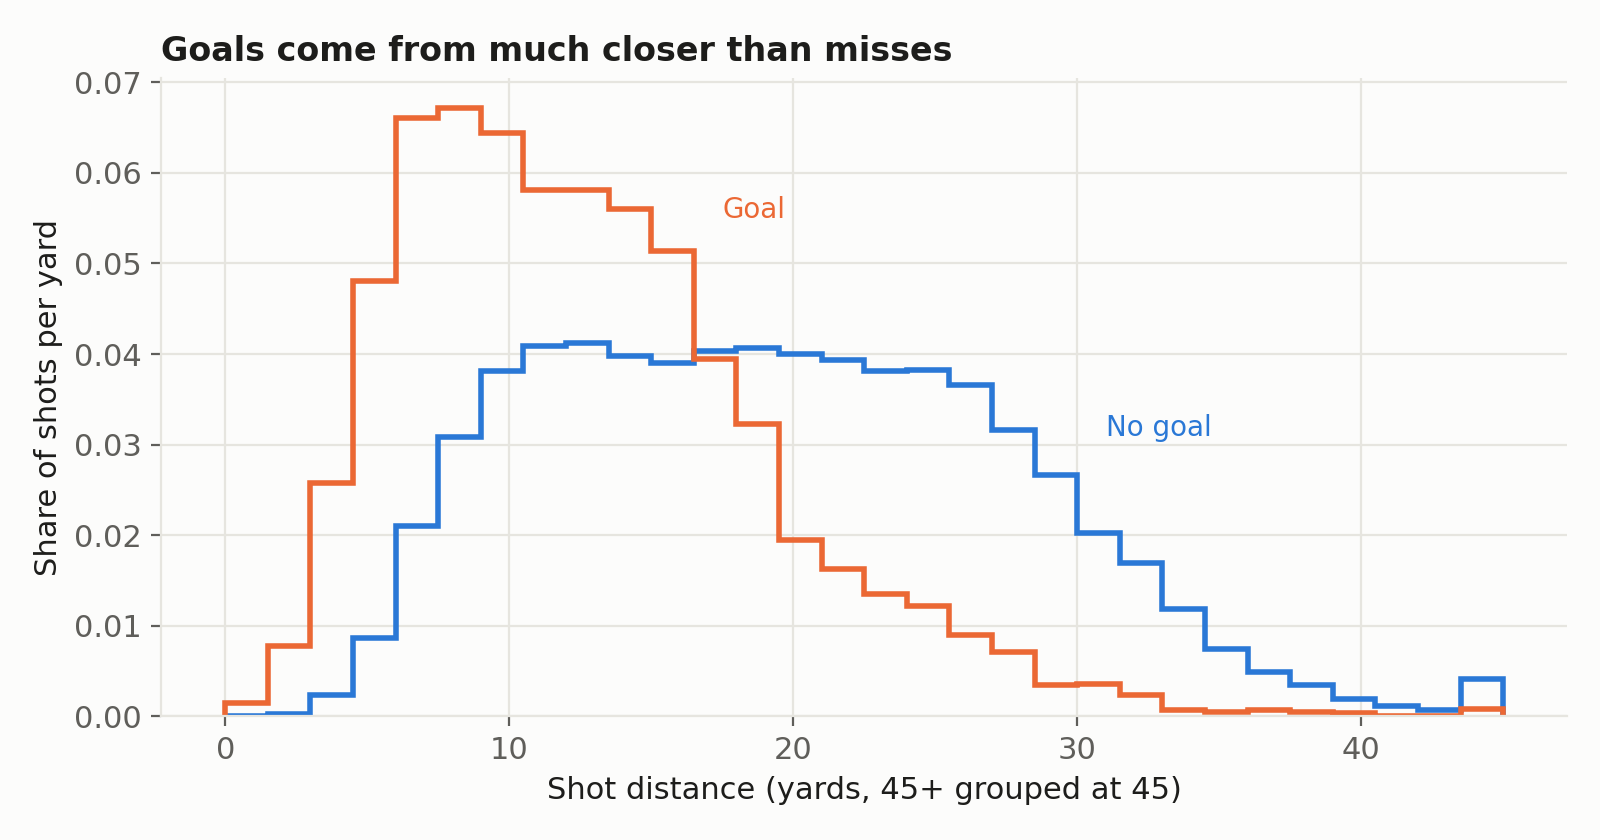
\includegraphics[width=0.9\textwidth]{images/histo.png}
    \caption{Shot Distance of Goals and Misses}
    \label{histo}
\end{figure}

88\% of goals were scored from inside the penalty area. Shot distance was therefore taken as a critical feature.

\newpage

\subsection{Shot Angle}\label{shotanglesec}

Consider the triangle formed by the shot location and the two goal posts. The Shot Angle is the angle of this triangle at the shot location, marked by the blue dot in figure \ref{shotangle}. The wider the angle, the more of the goal the shooter can see.

\begin{figure}[!h]
    \centering
    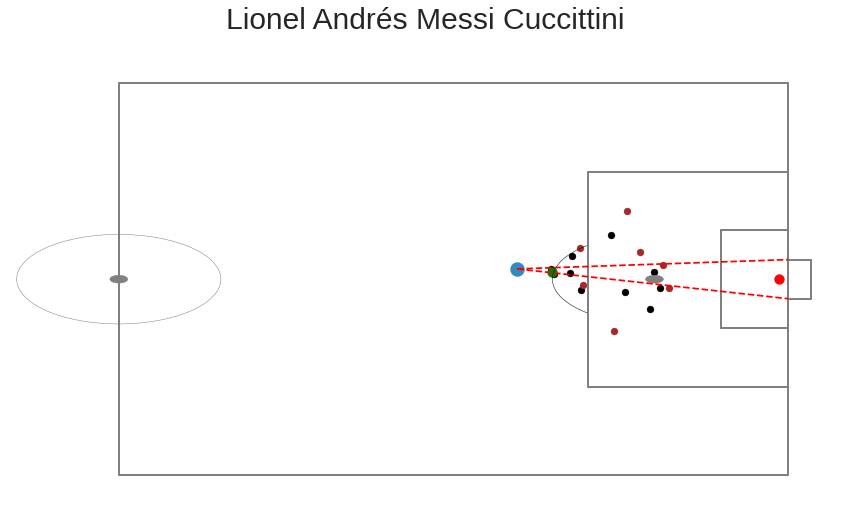
\includegraphics[scale=0.45]{images/messihalf.png}
    \caption{Shot Angle}
    \label{shotangle}
\end{figure}

Goals were scored from a median angle of 31.8°, against 19.1° for shots that did not result in a goal (figure \ref{shotangleplot}). The angle is closely related to distance, since shots from close in see more of the goal, but it also separates central shots from shots at the same distance from a tight angle.

\begin{figure}[!h]
    \centering
    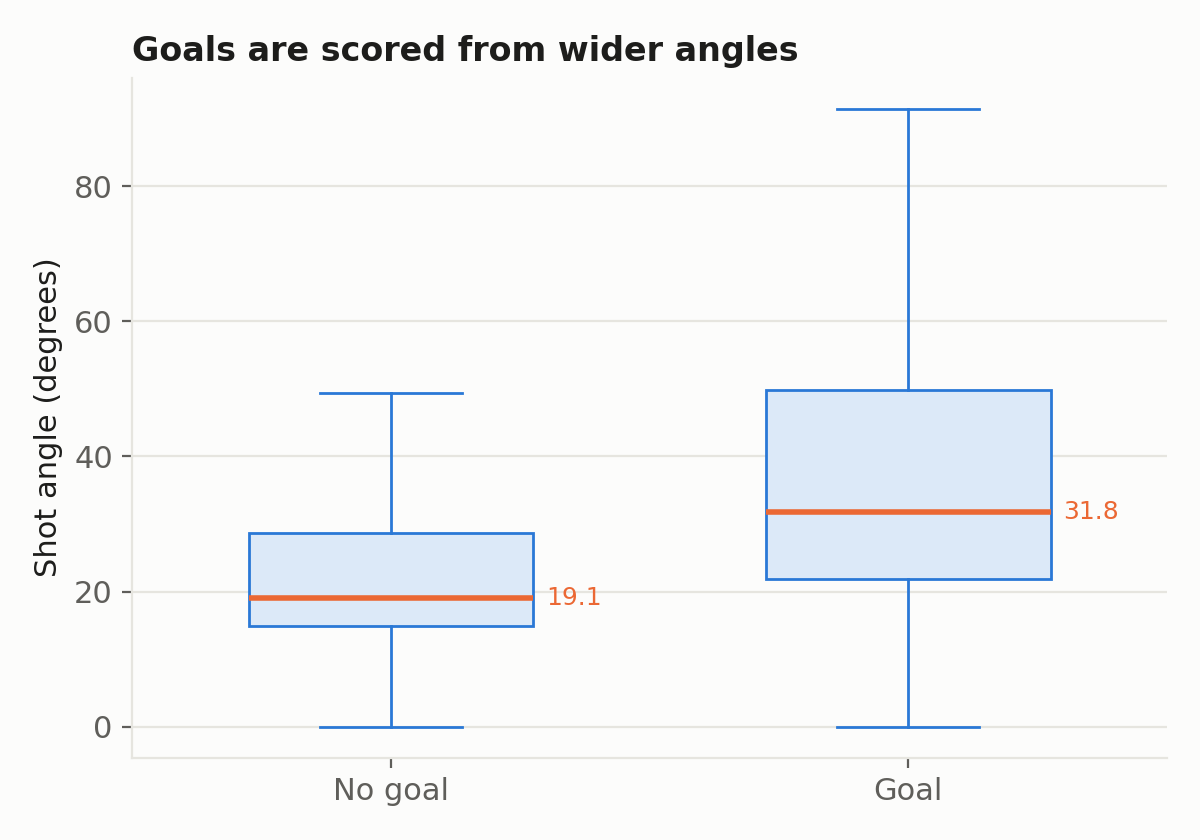
\includegraphics[width=0.6\textwidth]{images/angle1.png}
    \caption{Shot Angle of Goals and Misses (box plots without outliers)}
    \label{shotangleplot}
\end{figure}

\newpage

\subsection{Body Part}\label{bod}

There are two body parts that footballers use to shoot: the feet and the head. Any other body part is rare: only 154 of the 49,148 open-play shots in the training matches (0.3\%), and these were left out of the model (figure \ref{body}).

\begin{figure}[!h]
    \centering
    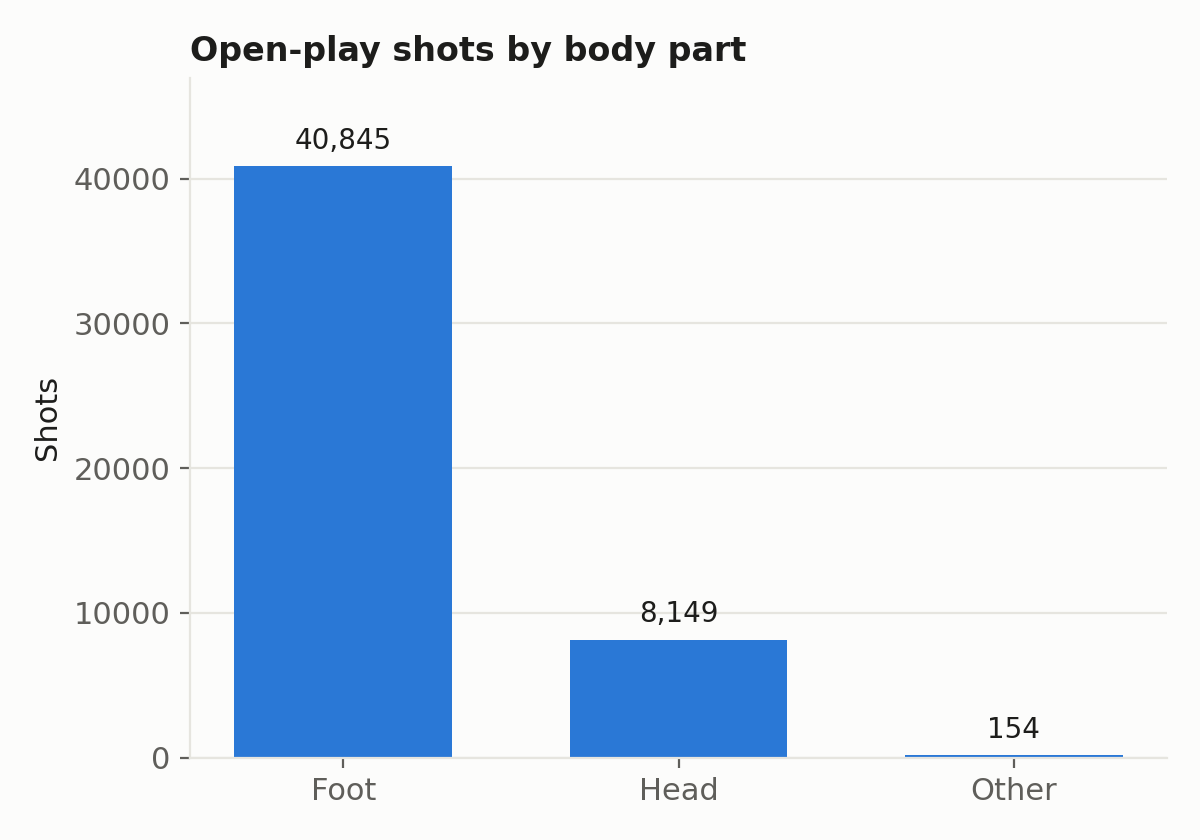
\includegraphics[width=0.6\textwidth]{images/body.png}
    \caption{Shots by Body Part}
    \label{body}
\end{figure}

Taken over all distances, shots with the foot and the head convert at almost the same rate: 10.2\% and 10.4\% (figure \ref{beforeskew}).

\begin{figure}[!h]
    \centering
    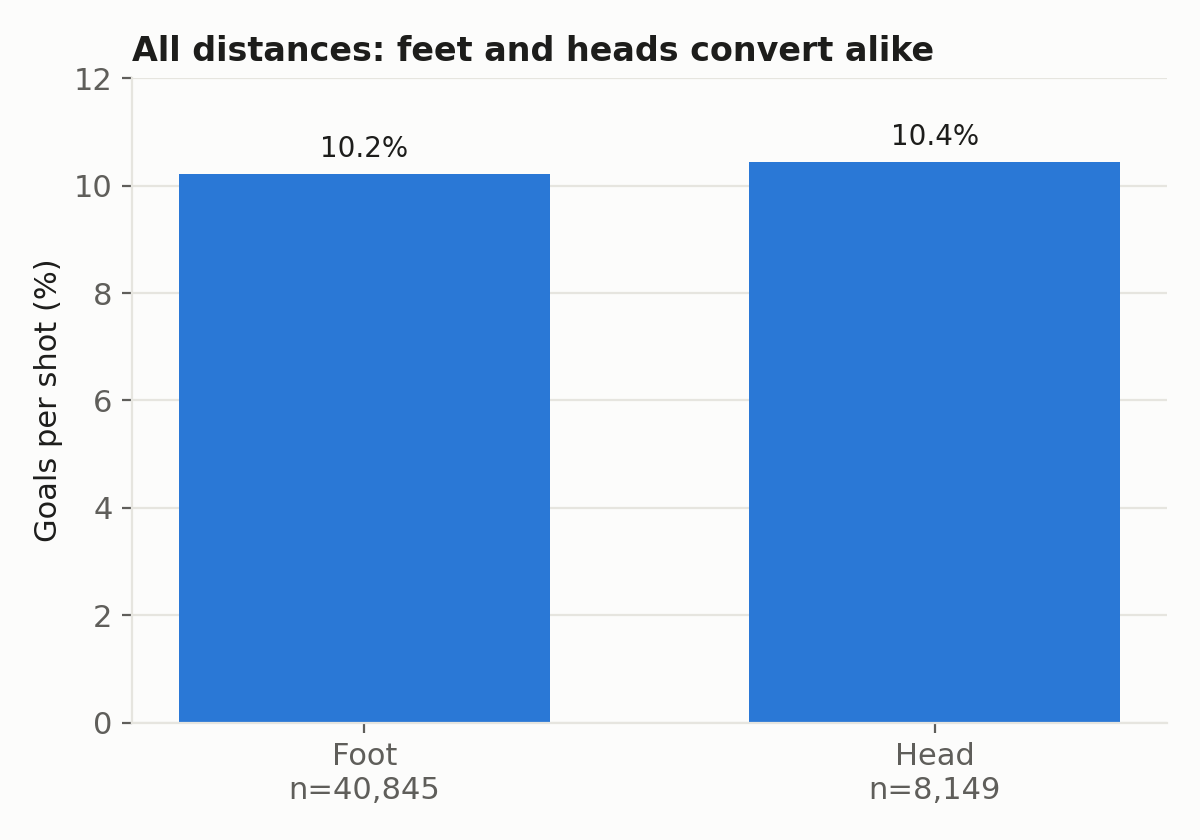
\includegraphics[width=0.6\textwidth]{images/beforeskew.png}
    \caption{Goals by Body Part, all Distances}
    \label{beforeskew}
\end{figure}

This comparison is misleading, because headers are taken much closer to goal. The median header is taken from 9.7 yards and the median shot with the foot from 20.3 yards, and 99\% of headers are taken from within 18 yards (figure \ref{bodybox}).

\begin{figure}[!h]
    \centering
    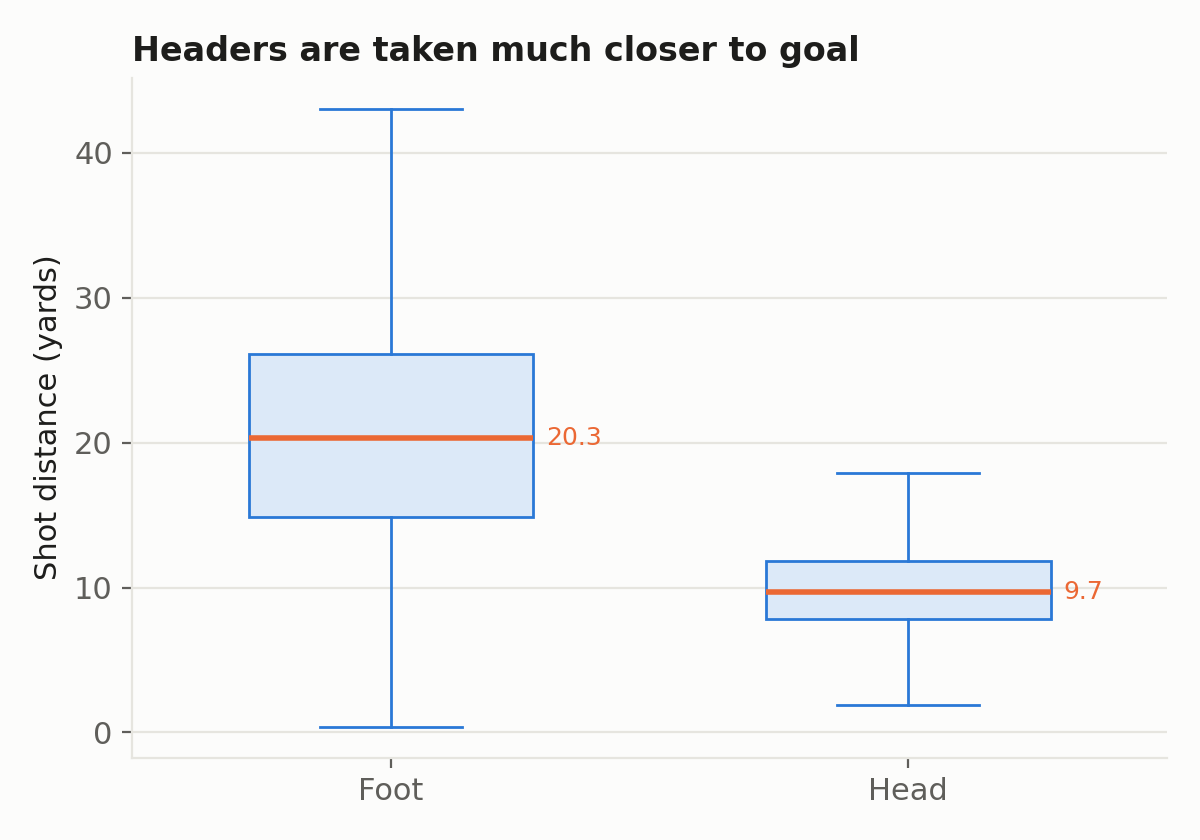
\includegraphics[width=0.6\textwidth]{images/bodybox.png}
    \caption{Shot Distance by Body Part (box plots without outliers)}
    \label{bodybox}
\end{figure}

When shots are compared at the same distance, the difference is large (figure \ref{afterskew}). Within 18 yards, 20.3\% of shots with the foot were goals, against 10.5\% of headers; under 12 yards the rates are 31.0\% and 12.5\%. As the hypothesis expected, a header is a much worse chance than a shot with the foot from the same place.

\begin{figure}[!h]
    \centering
    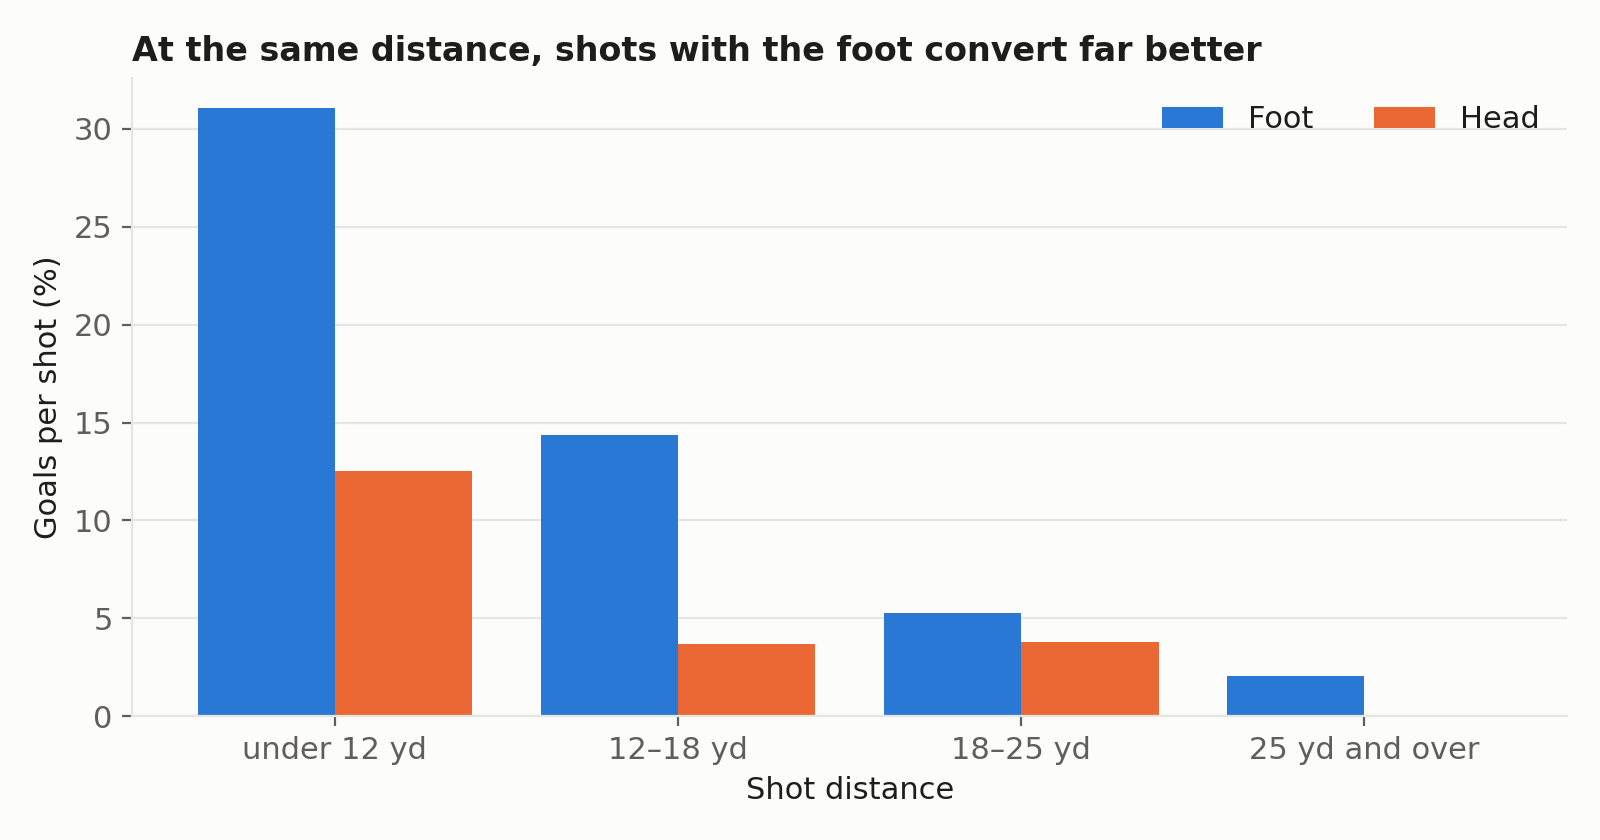
\includegraphics[width=0.9\textwidth]{images/afterskew.png}
    \caption{Goals by Body Part within Distance Bands}
    \label{afterskew}
\end{figure}

\newpage

\subsection{Pressure}\label{pressure}

When a player shoots, defenders close by can block the shot or hurry it. This was measured as the number of opponents within 5 yards of the shooter in the freeze frame.

Taken over all distances, pressure seems to make no difference: shots with 0, 1, 2 and 3 or more opponents within 5 yards convert at 9.9\%, 10.7\%, 10.0\% and 10.1\%. The reason is again distance. Pressure increases as the shot gets closer to goal: the median shot with no opponent nearby is taken from 24.8 yards, and with 3 or more from 12.8 yards (figure \ref{5yardsbox}).

\begin{figure}[!h]
    \centering
    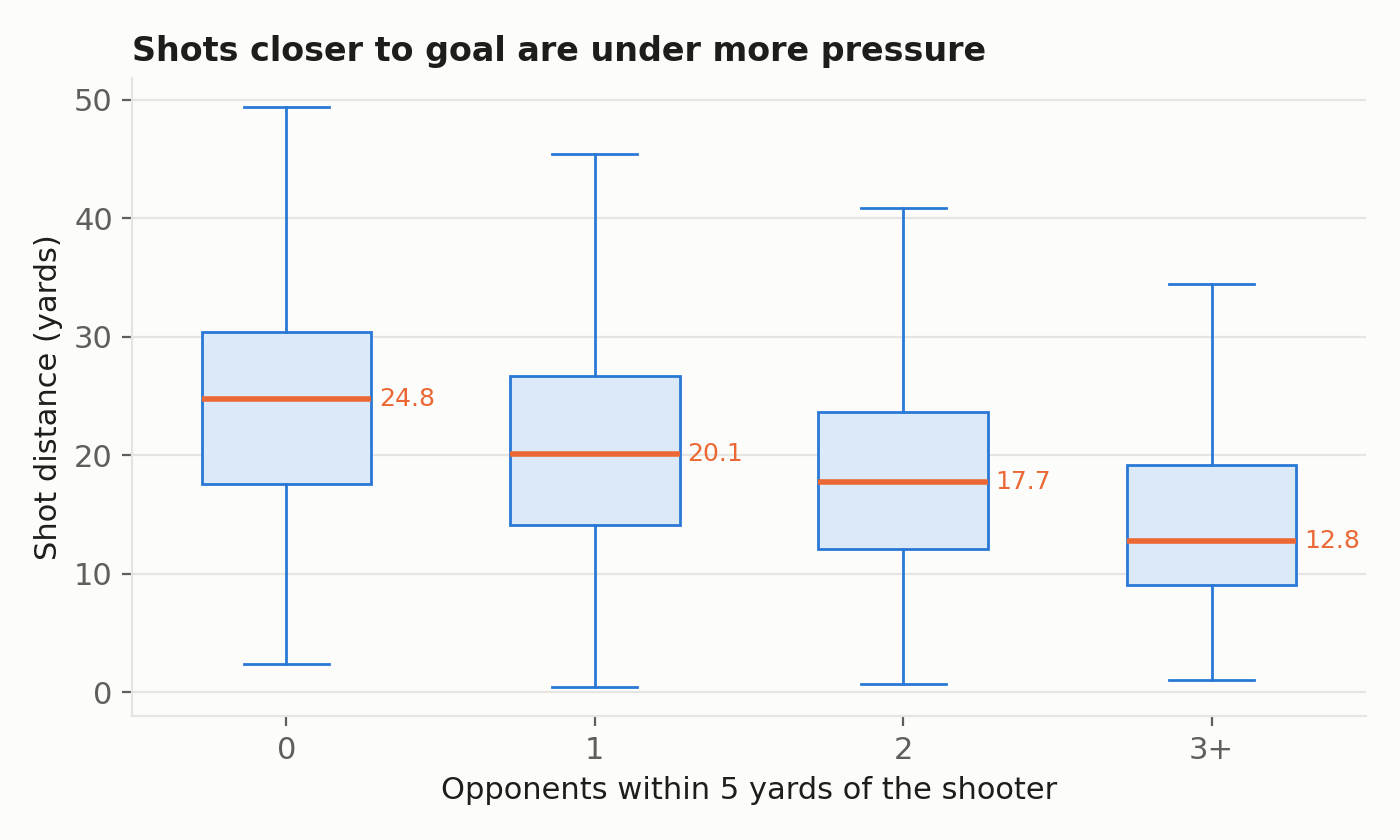
\includegraphics[width=0.75\textwidth]{images/5yardsbox.png}
    \caption{Shot Distance vs Pressure (box plots without outliers)}
    \label{5yardsbox}
\end{figure}

Within each distance band, the hypothesis holds (figure \ref{5yardsbar}). Under 12 yards, the goal rate falls from 40.9\% with no opponent nearby to 29.6\%, 21.4\% and 14.2\% with 1, 2 and 3 or more. The effect is smaller for long shots, which rarely go in whatever the pressure.

\begin{figure}[!h]
    \centering
    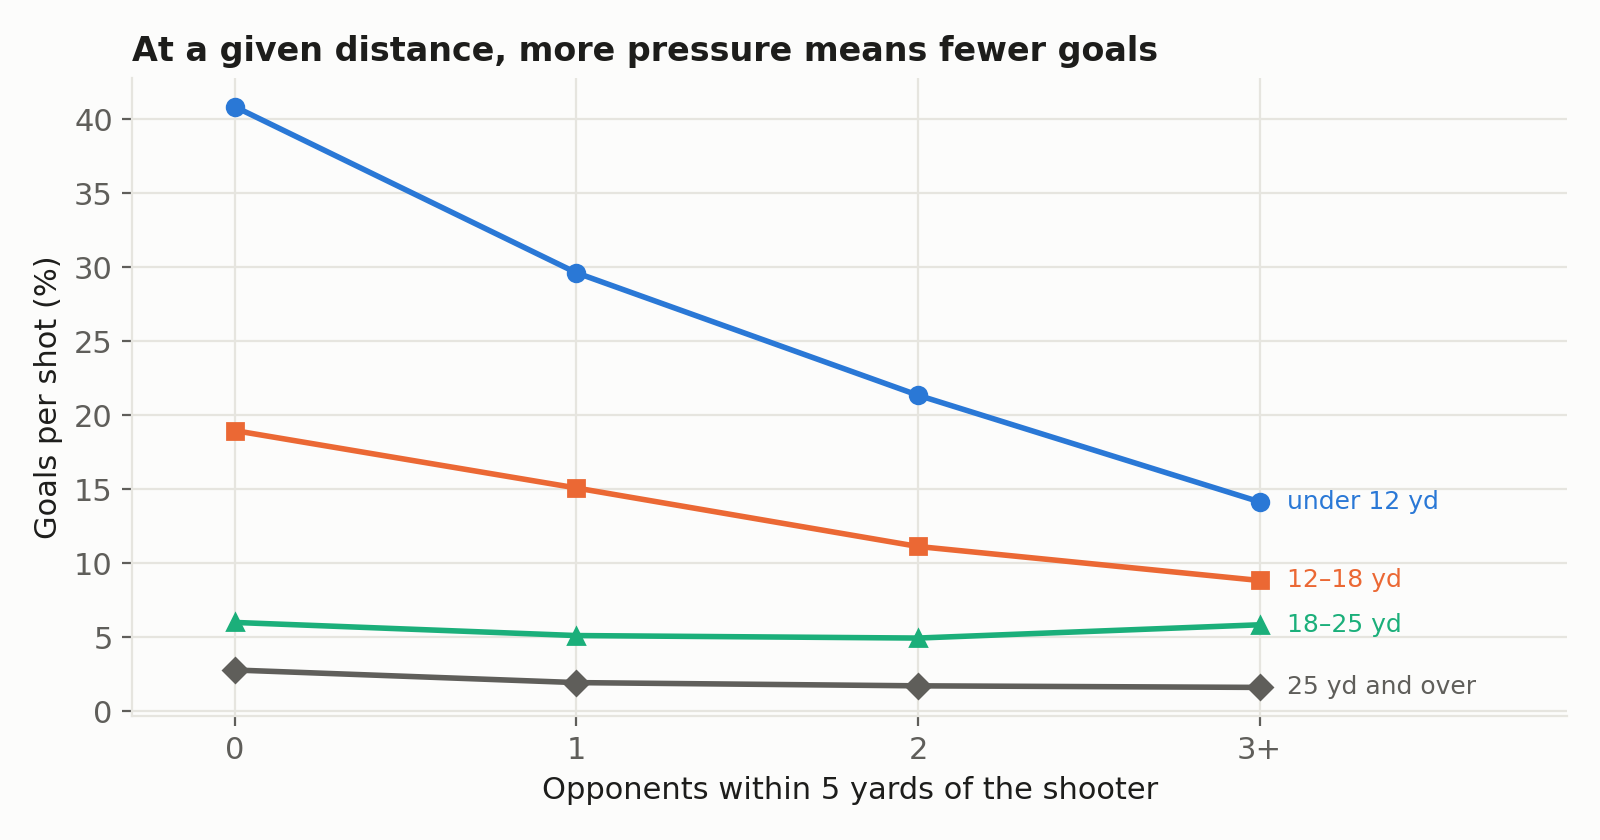
\includegraphics[width=0.9\textwidth]{images/5yardsbar.png}
    \caption{Goal Percentage vs Pressure within Distance Bands}
    \label{5yardsbar}
\end{figure}

\newpage

\subsection{Number of Players in front of Goal}

Consider again the triangle formed by the shot location and the two posts (figure \ref{shotangle}). Opponents inside this triangle, including the goalkeeper, stand between the ball and the goal and can block the shot (figure \ref{messi}). The number of opponents inside the triangle was counted from the freeze frame.

\begin{figure}[!h]
    \centering
    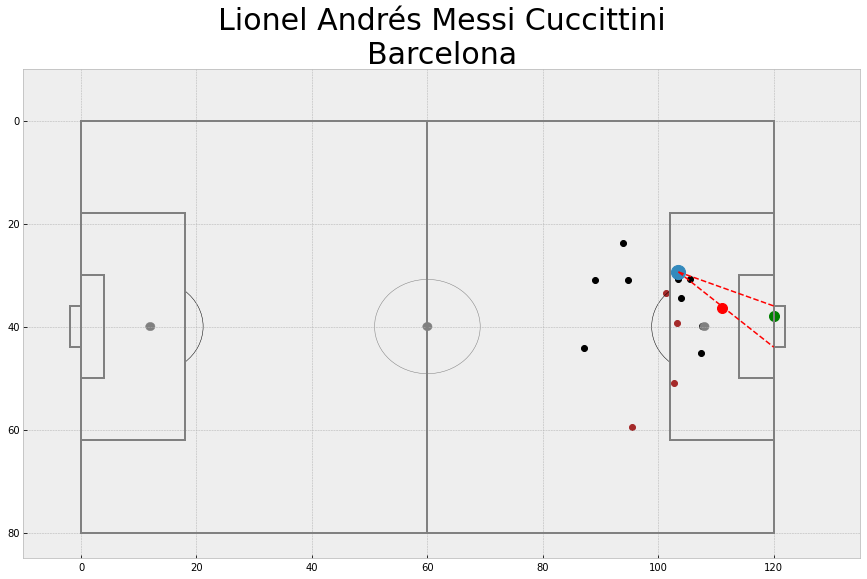
\includegraphics[scale=0.5]{images/messsiiii.png}
    \caption{Players between Goal}
    \label{messi}
\end{figure}

This feature has the strongest relation with goals of all the freeze-frame features (figure \ref{oppobtngoal}). With nobody in the triangle, which usually means the goalkeeper has been beaten or drawn out, 43.8\% of shots were goals. With one player in the way, usually only the goalkeeper, the rate was 13.0\%, and it fell to 5.8\%, 4.4\% and 3.5\% with 2, 3 and 4 or more.

\begin{figure}[!h]
    \centering
    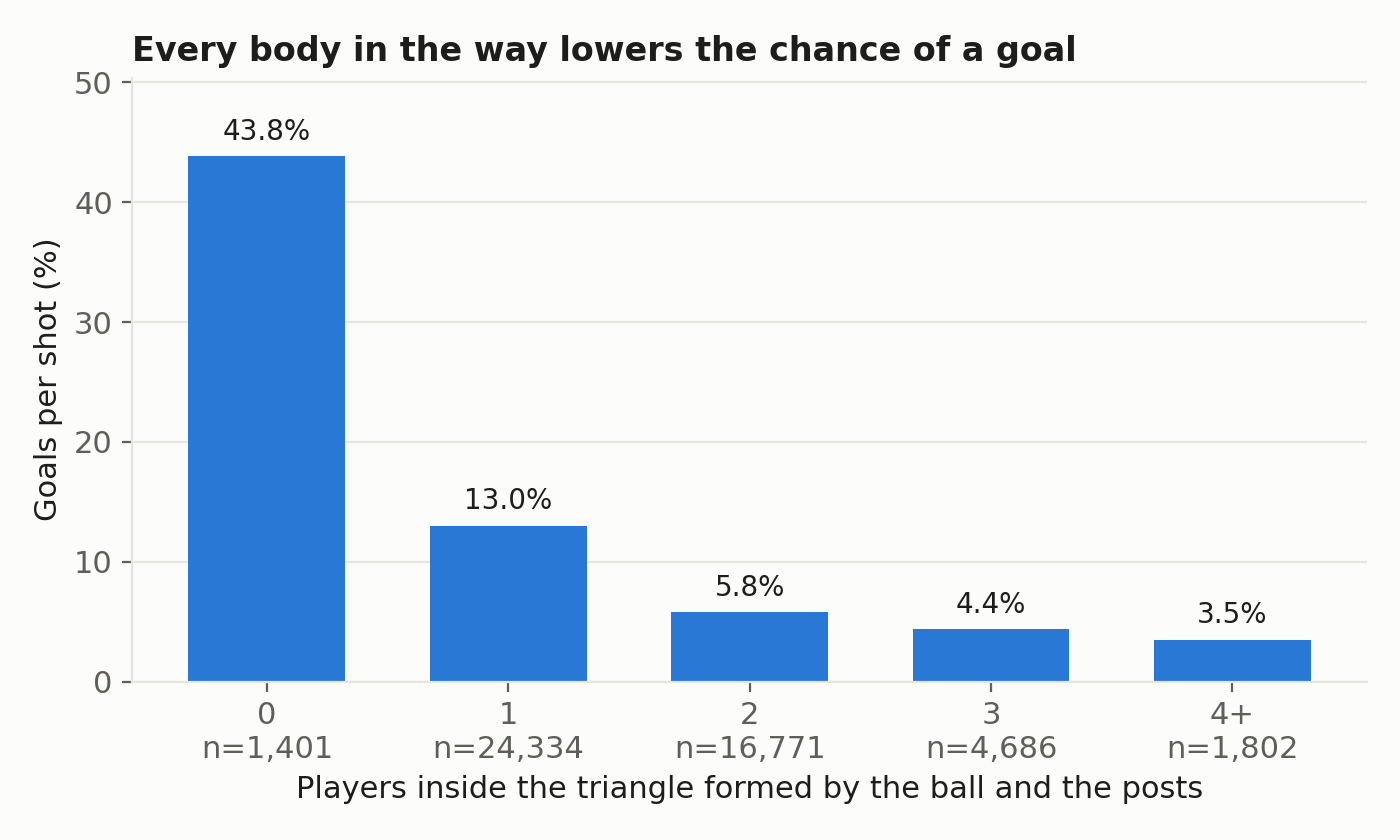
\includegraphics[width=0.75\textwidth]{images/opponentsbetweengoalbar.png}
    \caption{Goal Percentage vs Players between Ball and Goal}
    \label{oppobtngoal}
\end{figure}

The number of players in the way rises with distance, from a median distance of 9.9 yards with nobody in the triangle to about 21 yards with 3 or more (figure \ref{oppobtngoalbox}), since a longer shot passes through more of the pitch. Distance, angle and the players in the way therefore add up: a long shot from a tight angle through a crowded area has an xG close to zero.

\begin{figure}[!h]
    \centering
    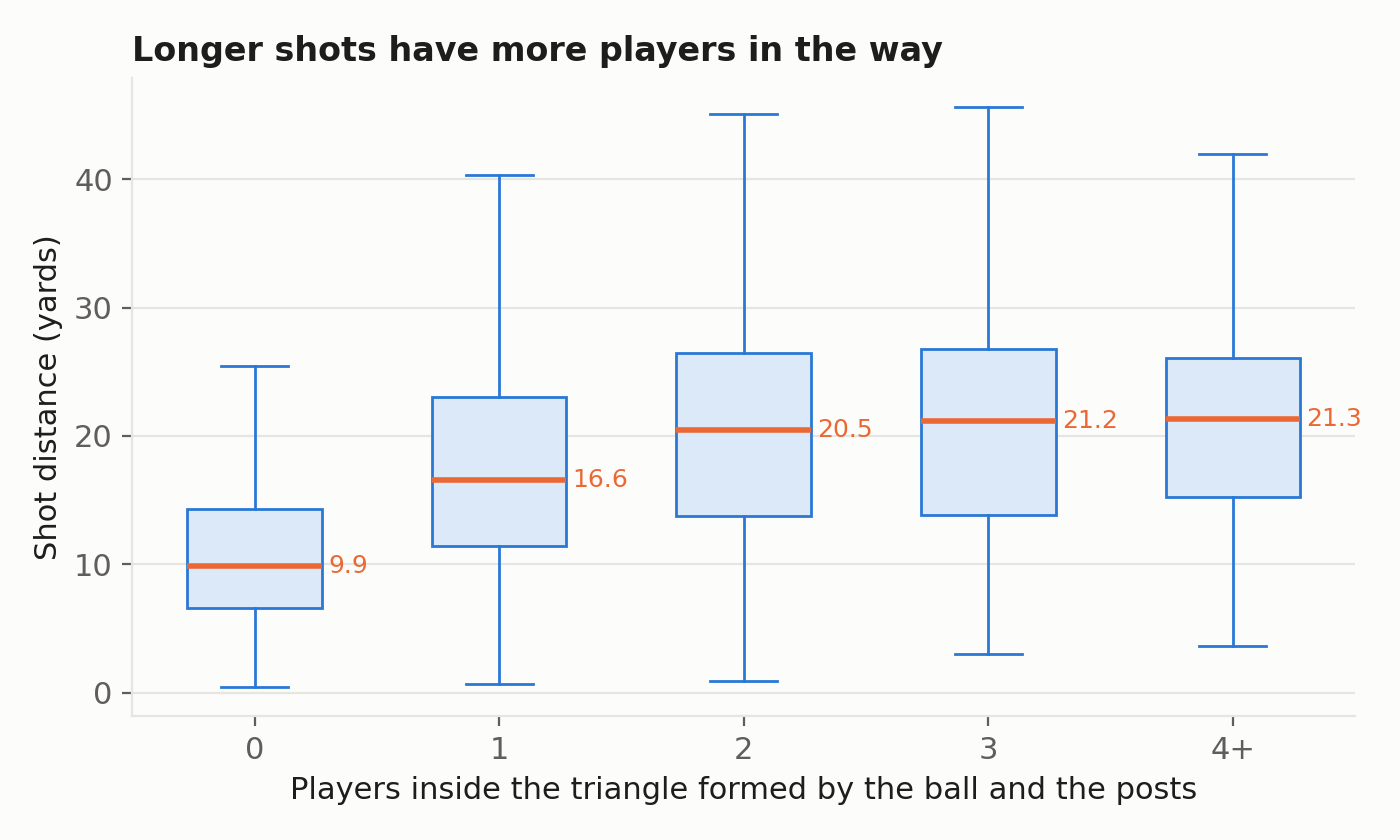
\includegraphics[width=0.75\textwidth]{images/opponentsgoalbox.png}
    \caption{Shot Distance vs Players between Ball and Goal (box plots without outliers)}
    \label{oppobtngoalbox}
\end{figure}

\newpage

\subsection{Goal Keeper Distance and Location}

Though a goalkeeper stays near the goal for most of a match, there are situations when he or she has to move away from it. In a one-on-one, for example, goalkeepers come towards the striker to narrow the angle. The goalkeeper's distance from the centre of the goal was therefore analysed.

\begin{figure}[!h]
    \centering
    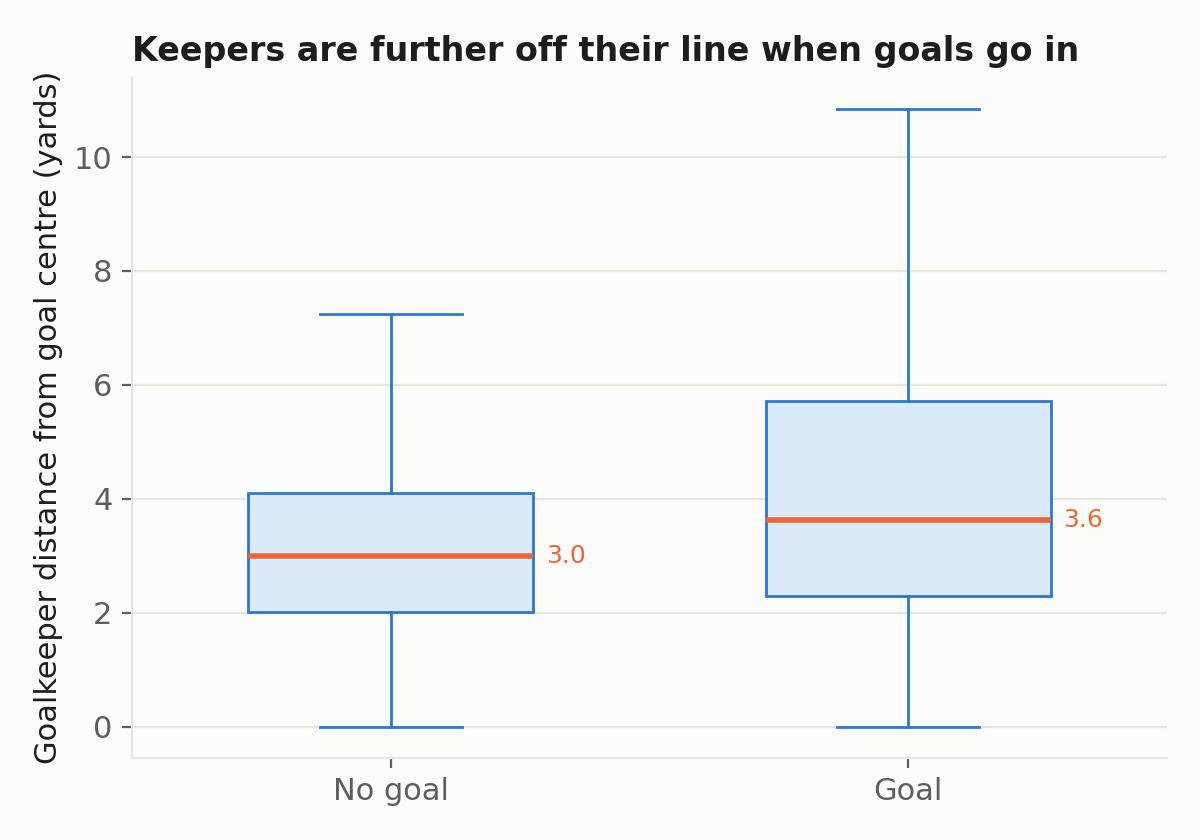
\includegraphics[width=0.6\textwidth]{images/gkdist.png}
    \caption{Goal Keeper Distance for Goals and Misses (box plots without outliers)}
    \label{gkdist}
\end{figure}

As the hypothesis proposed, goalkeepers were further from their goal when goals were scored: a median of 3.6 yards against 3.0 yards, and a mean of 4.6 yards against 3.4 yards (figure \ref{gkdist}).

\begin{figure}[!h]
    \centering
    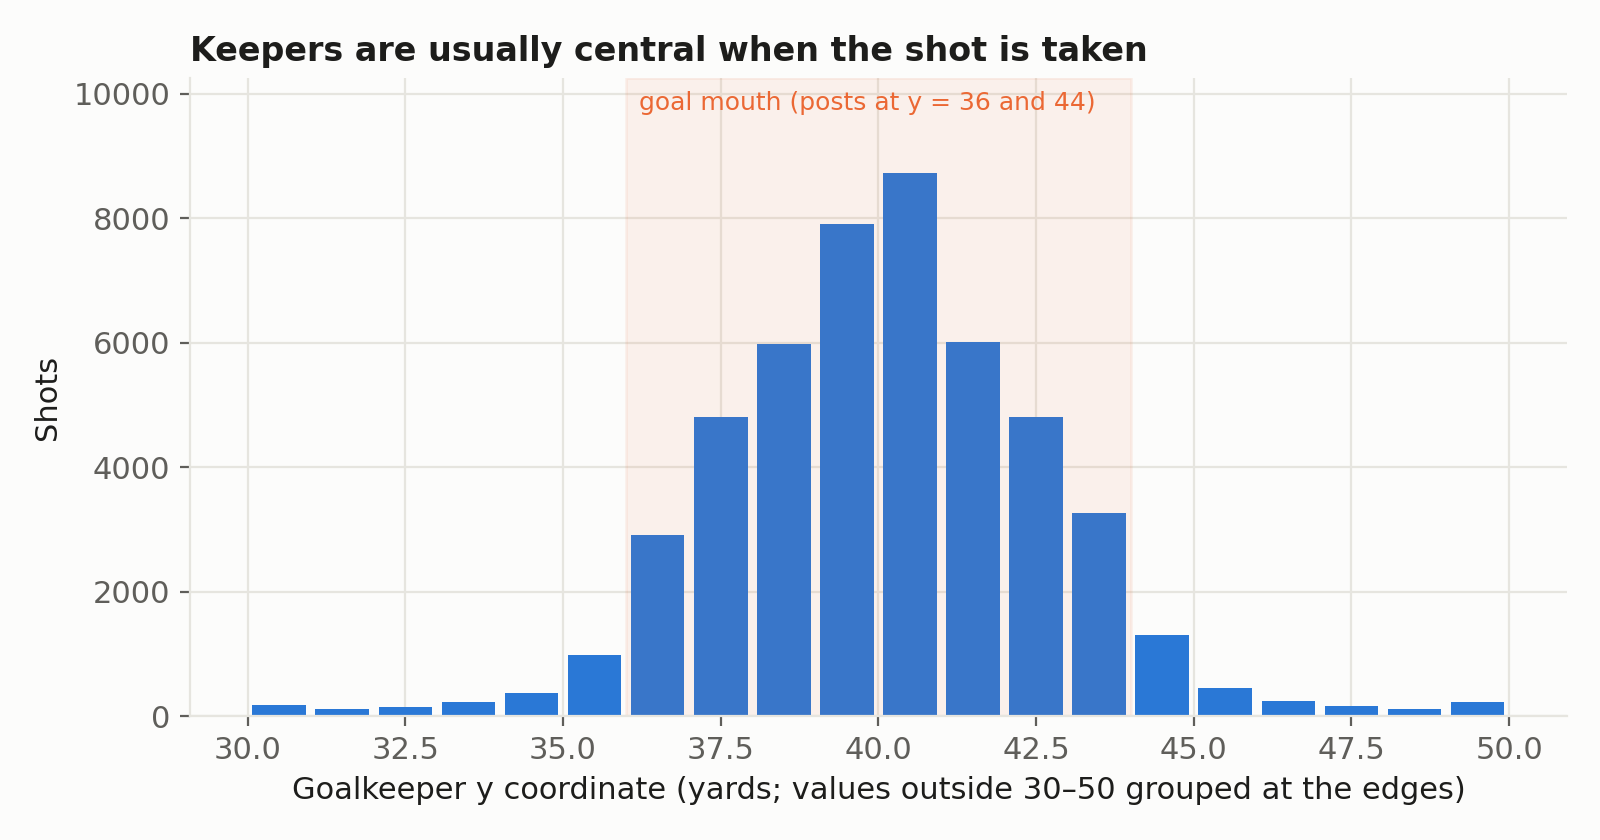
\includegraphics[width=0.9\textwidth]{images/ygkloc.png}
    \caption{Goal Keeper Y Coordinate at the Moment of the Shot}
    \label{ygkloc}
\end{figure}

The goalkeeper's y coordinate shows where they stand across the goal. Most shots were taken with the goalkeeper near the centre of the goal: in 60\% of shots the goalkeeper stood between $y = 38$ and $y = 42$ (figures \ref{ygkloc} and \ref{gkloc}). The goalkeeper's x and y coordinates were both included in the model.

\begin{figure}[!h]
    \centering
    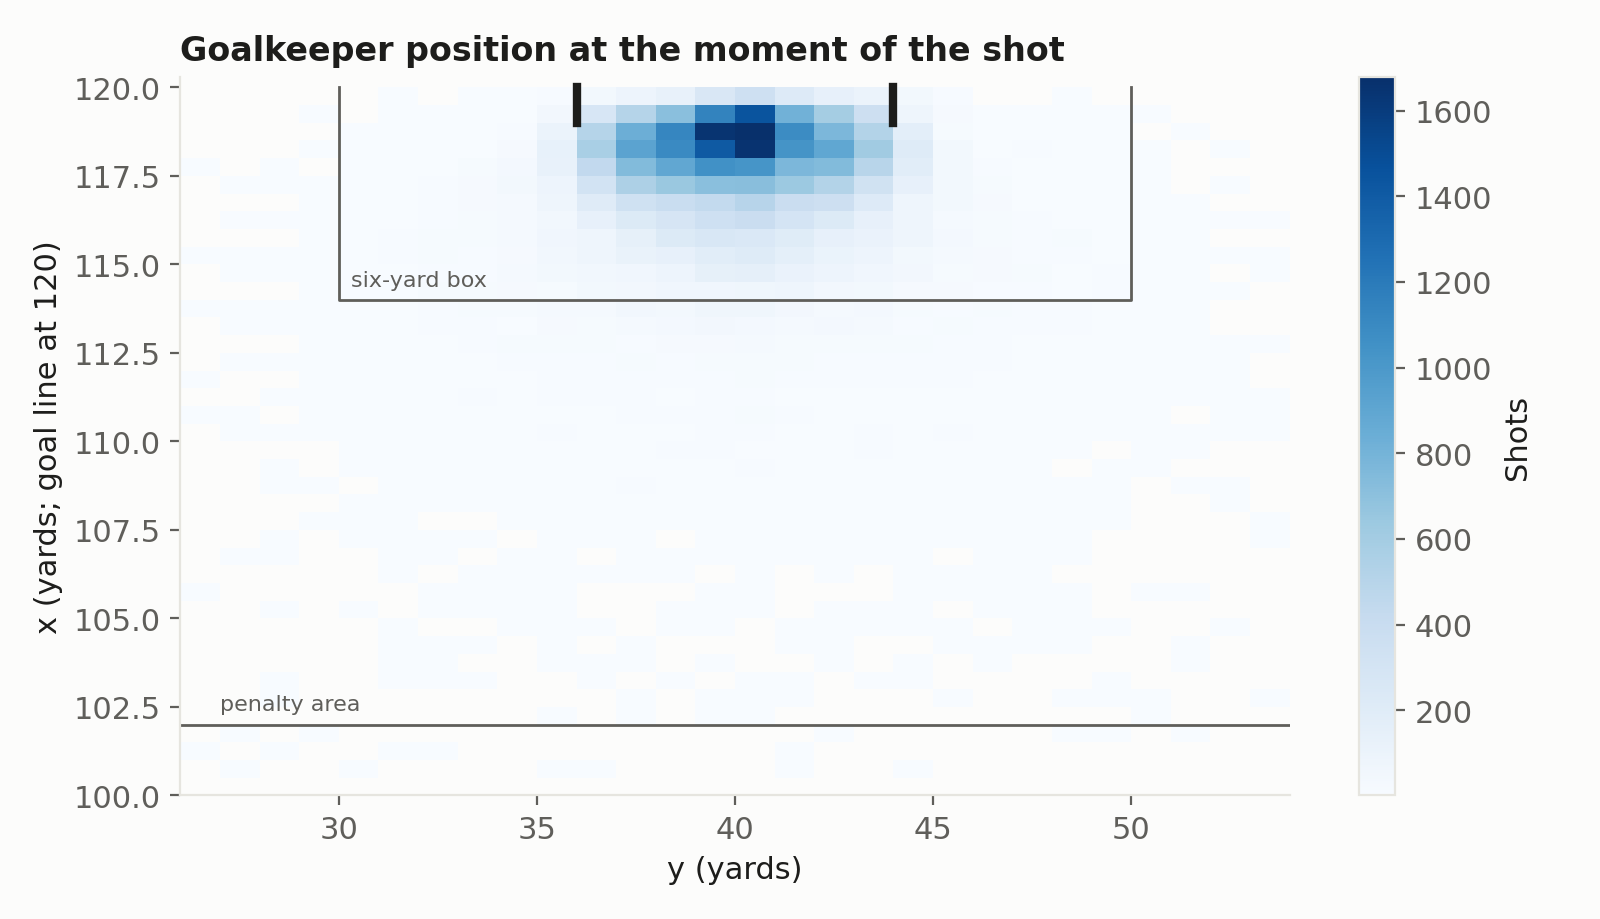
\includegraphics[width=0.9\textwidth]{images/gkloc.png}
    \caption{Goal Keeper Location at the Moment of the Shot}
    \label{gkloc}
\end{figure}

\newpage

\subsection{Preceding Play Pattern}

The play pattern describes the passage of play that led to the shot. The play patterns defined by StatsBomb \cite{Statsbomb} are:

\begin{itemize}
    \item 'From Counter': The event was part of a counter attack:
    \begin{itemize}
        \item The possession began with an open play turnover outside the counter-attacking team’s final third.
        \item The possession was at least 75\% direct towards goal.
        \item The attack travelled a minimum of 18 yards towards goal.
    \end{itemize}
    \item 'From Throw In': The passage of play after a throw-in.
    \item 'Regular Play': None of the other play patterns.
    \item 'From Corner': The passage of play after a corner.
    \item 'From Free Kick': The passage of play after a free-kick.
    \item 'From Goal Kick': The passage of play after a goal kick.
    \item 'From Kick Off': The passage of play after the kick off.
    \item 'From Keeper': The passage of play after a keeper distribution.
\end{itemize}

These play patterns describe the build-up to an open-play shot; they must not be confused with direct shots from set pieces, which are not part of this model. Most shots come from regular play, followed by throw-ins, free kicks and corners (figure \ref{playpatt}).

\begin{figure}[!h]
    \centering
    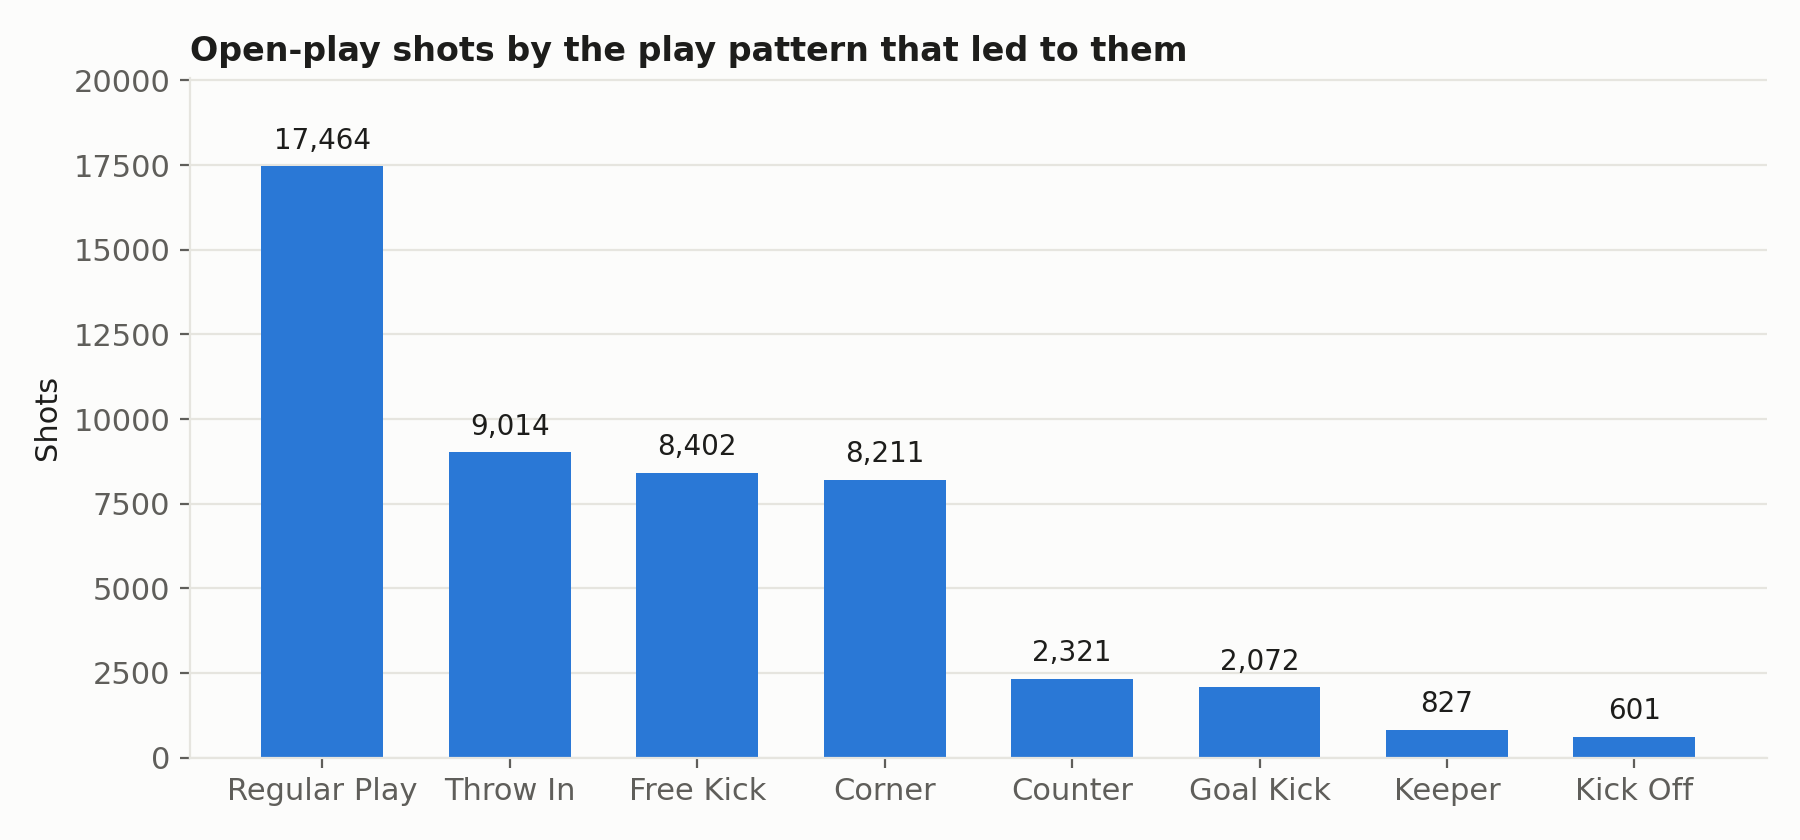
\includegraphics[width=0.9\textwidth]{images/playpatt.png}
    \caption{Shots by Play Pattern}
    \label{playpatt}
\end{figure}

\begin{figure}[!h]
    \centering
    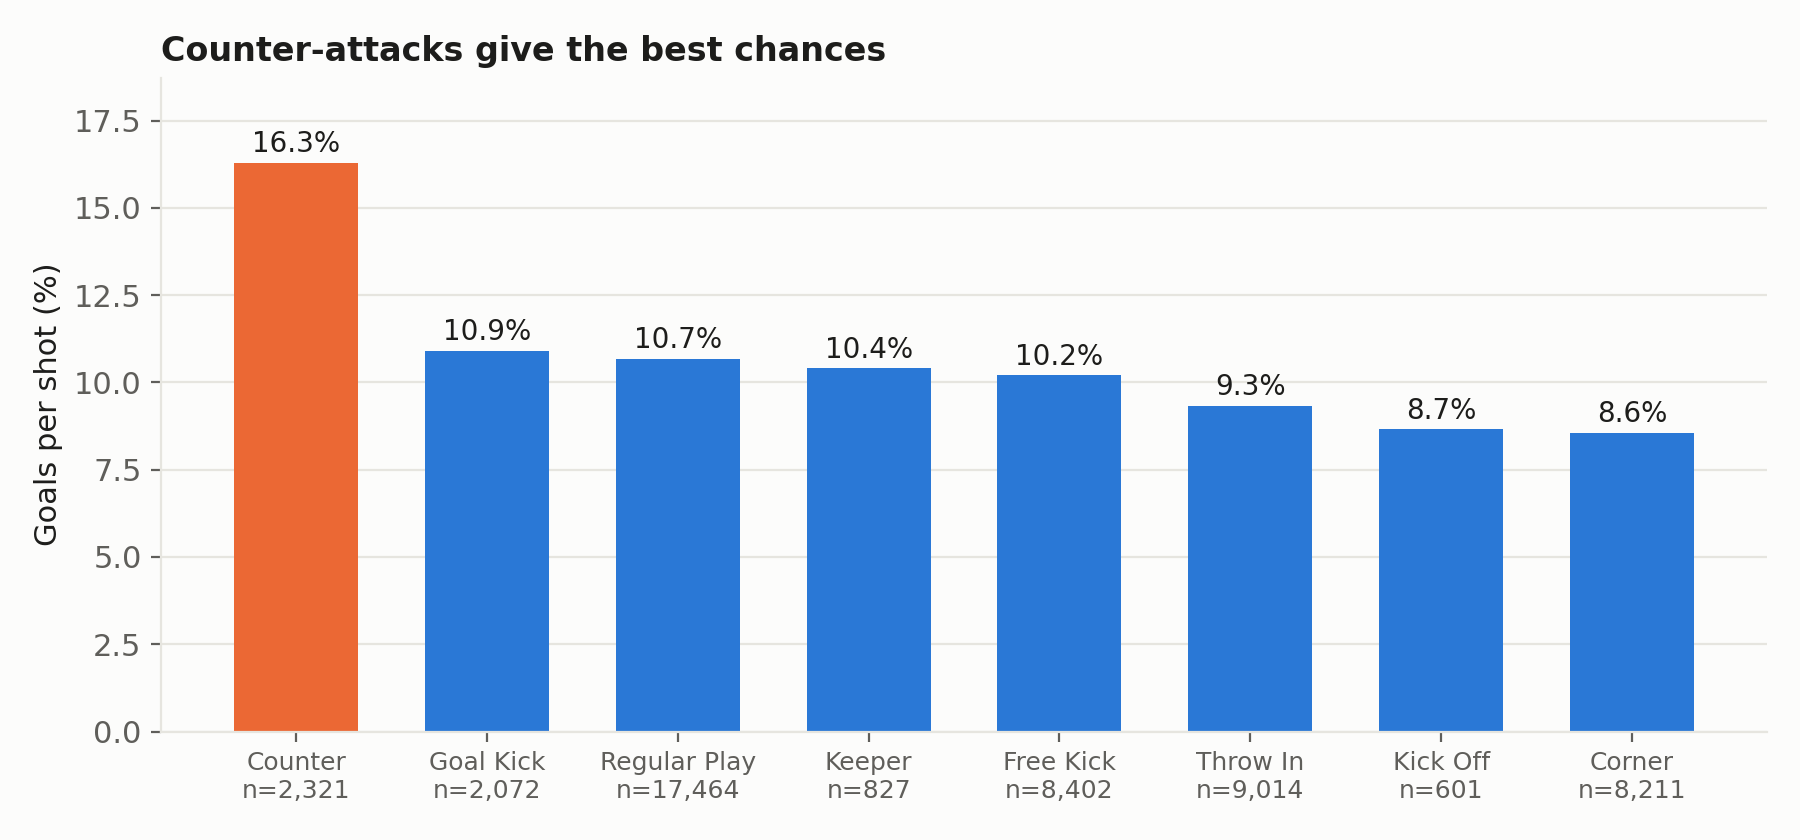
\includegraphics[width=0.9\textwidth]{images/playpattern.png}
    \caption{Goal Percentage by Play Pattern}
    \label{playpattern}
\end{figure}

Counter attacks stand out (figure \ref{playpattern}): 16.3\% of shots from counters were goals, against 8.6\%--10.9\% for every other pattern. Shots after corners and kick-offs converted least often (8.6\% and 8.7\%). The original edition stated that many goals came from kick-offs; on the wider data this does not hold, and kick-offs lead to few shots (1.2\%) that convert below average.

Following the original study, the model uses play pattern in two groups, Regular Play and Non Regular Play. Their goal rates differ little (10.7\% and 10.0\%), because the grouping mixes counters with corners. This is one of the reasons the play pattern ends up as the least useful feature (section \ref{res:importance}), and a finer grouping that keeps counter attacks apart is suggested as future work.

\newpage

\subsection{Pass Type and Ball Height}

The key pass before a shot can be a ground pass, a low pass (in the air, below shoulder height) or a high pass. Some shots follow no pass at all, for example after a dribble or a rebound. The hypothesis was that ground and low passes lead to better chances than high passes.

\begin{figure}[!h]
    \centering
    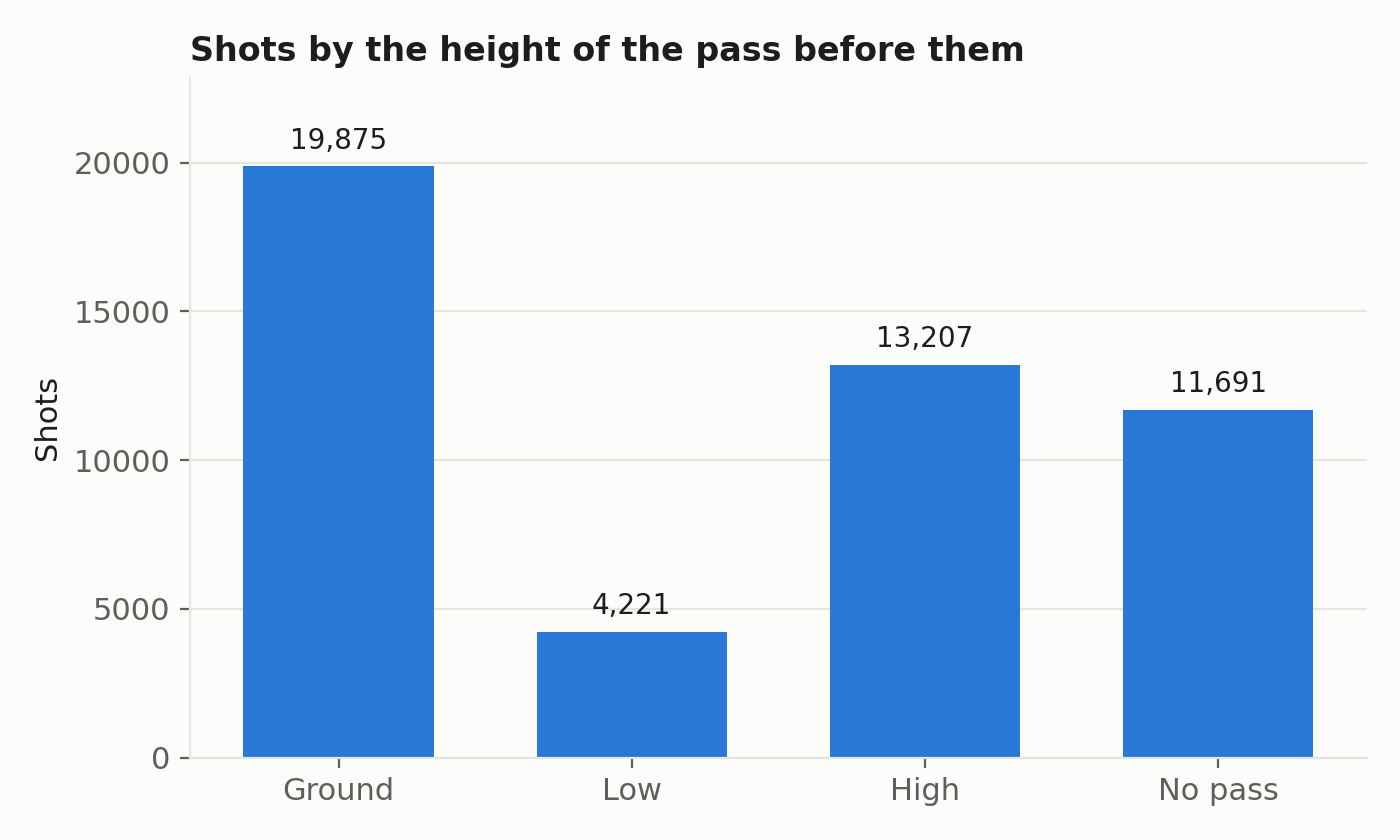
\includegraphics[width=0.7\textwidth]{images/passtypeshot.png}
    \caption{Shots by Pass Type}
    \label{passtypeshot}
\end{figure}

Ground passes and high passes created the most shots (figure \ref{passtypeshot}). High passes lead to shots much closer to goal, with a median of 11.4 yards against 21.7 yards after a ground pass (figure \ref{passtypebox}), because 57\% of the shots after a high pass are headers.

\begin{figure}[!h]
    \centering
    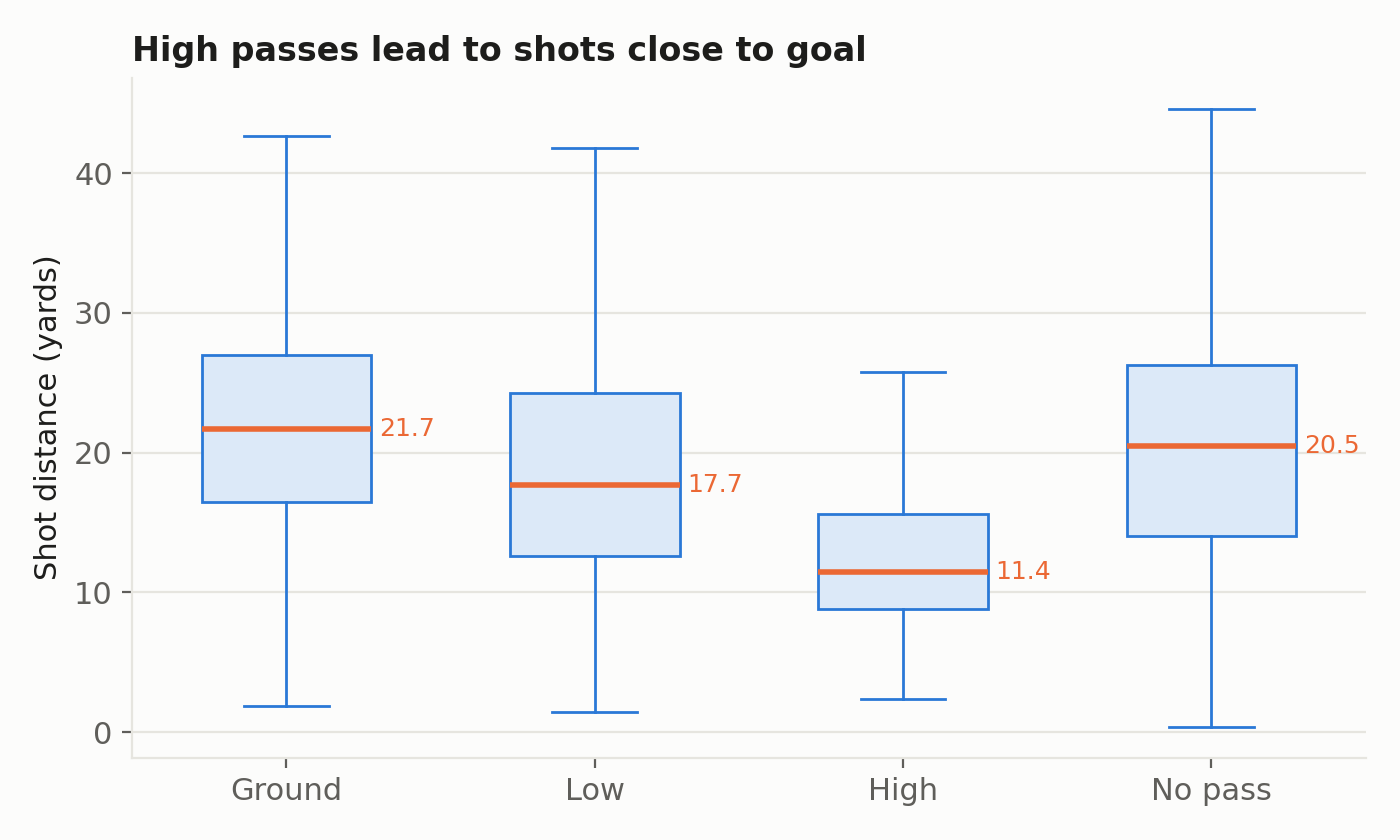
\includegraphics[width=0.7\textwidth]{images/passtypebox.png}
    \caption{Shot Distance by Pass Type (box plots without outliers)}
    \label{passtypebox}
\end{figure}

Over all distances, the goal rates differ little: 9.7\% after a ground pass, 11.9\% after a low pass, 10.3\% after a high pass and 10.5\% with no pass. At the same distance, the hypothesis holds clearly (figure \ref{passtypeperc}). Under 12 yards, 37.5\% of shots after a ground pass were goals, but only 13.7\% of shots after a high pass. The ball arriving in the air, and often having to be headed, makes the chance much harder.

\begin{figure}[!h]
    \centering
    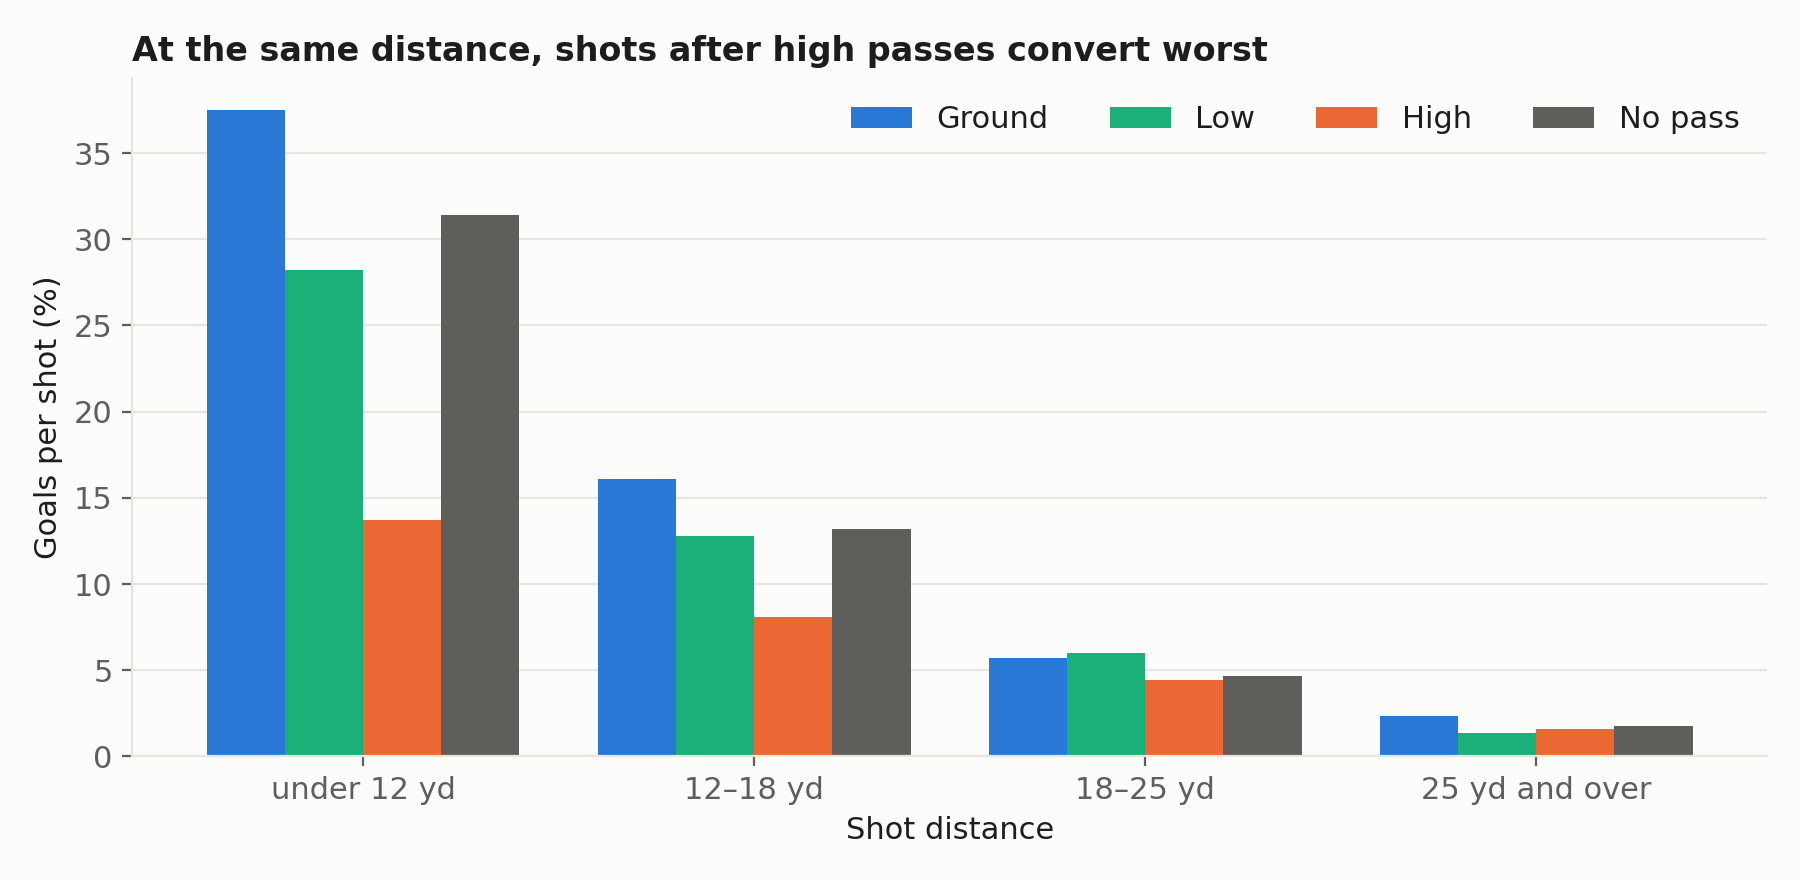
\includegraphics[width=0.9\textwidth]{images/passtypeperc.png}
    \caption{Goal Percentage by Pass Type within Distance Bands}
    \label{passtypeperc}
\end{figure}

\newpage

\subsection{Direct Goals From Set Pieces}

A set piece restarts play after a foul or after the ball has gone out of play: corners, free kicks and penalties \cite{washington}. Shots taken directly from a free kick or a penalty are very different chances from open-play shots. Penalties are usually given a fixed xG of about 0.76--0.79, and direct free kicks are modelled separately. This model therefore covers open-play shots only.

\subsection{First Time Shot}

A first-time shot is struck with the player's first touch, giving the defence and the goalkeeper less time to react. The hypothesis was that first-time shots have a higher xG, and it held: 14.0\% of first-time shots were goals against 8.4\% of the others (figure \ref{firstime}). The difference is largest close to goal: under 12 yards, 31.3\% against 16.0\%.

\begin{figure}[!h]
    \centering
    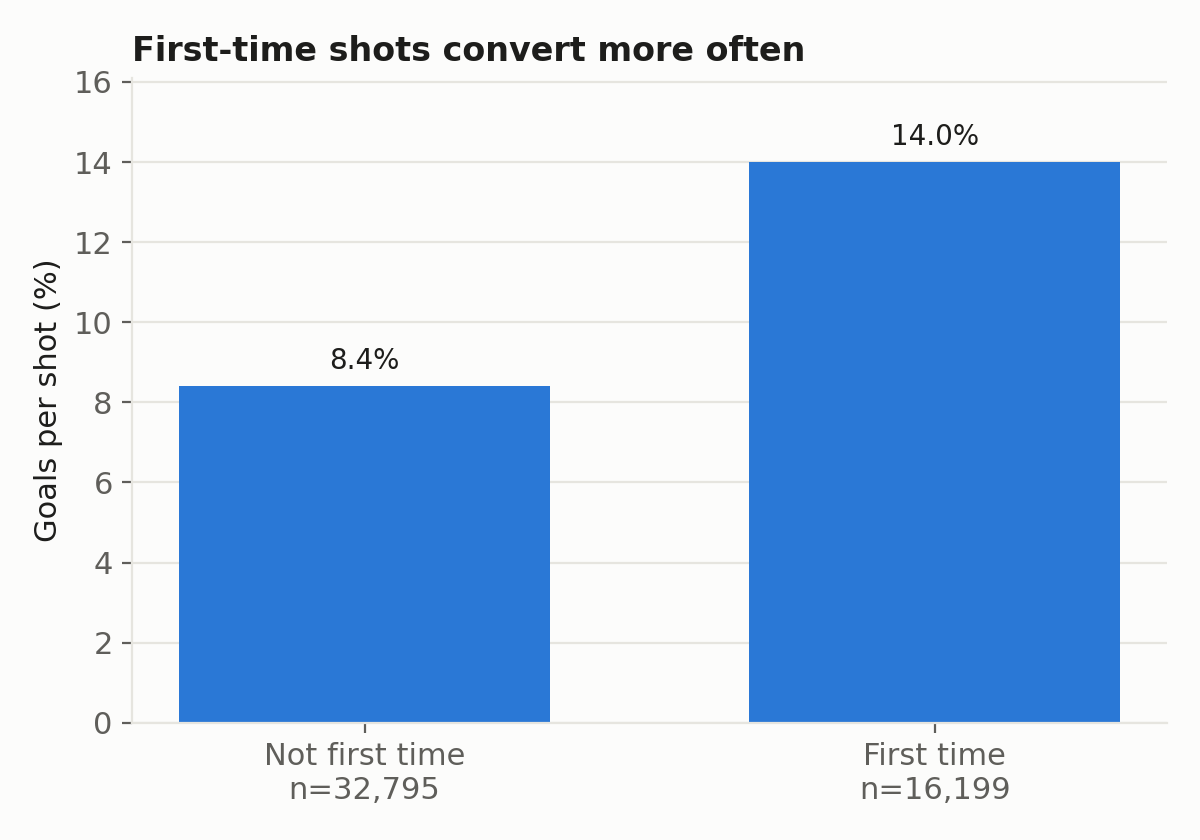
\includegraphics[width=0.6\textwidth]{images/firsttimeperc.png}
    \caption{Goals vs First Time Shots}
    \label{firstime}
\end{figure}

\newpage

\subsection{Technique Used and Shot Velocity}

The technique used to strike the ball, and the speed of the shot, say a lot about shot quality. Both were left out of the model on purpose. Expected Goals measures the quality of a chance \textbf{before} the shot is taken (\textbf{pre-shot analysis}), and the technique and speed of a shot are part of how the chance was taken, not of the chance itself. Their use in post-shot models is discussed in section \ref{future}.

\begin{figure}[!h]
    \centering
    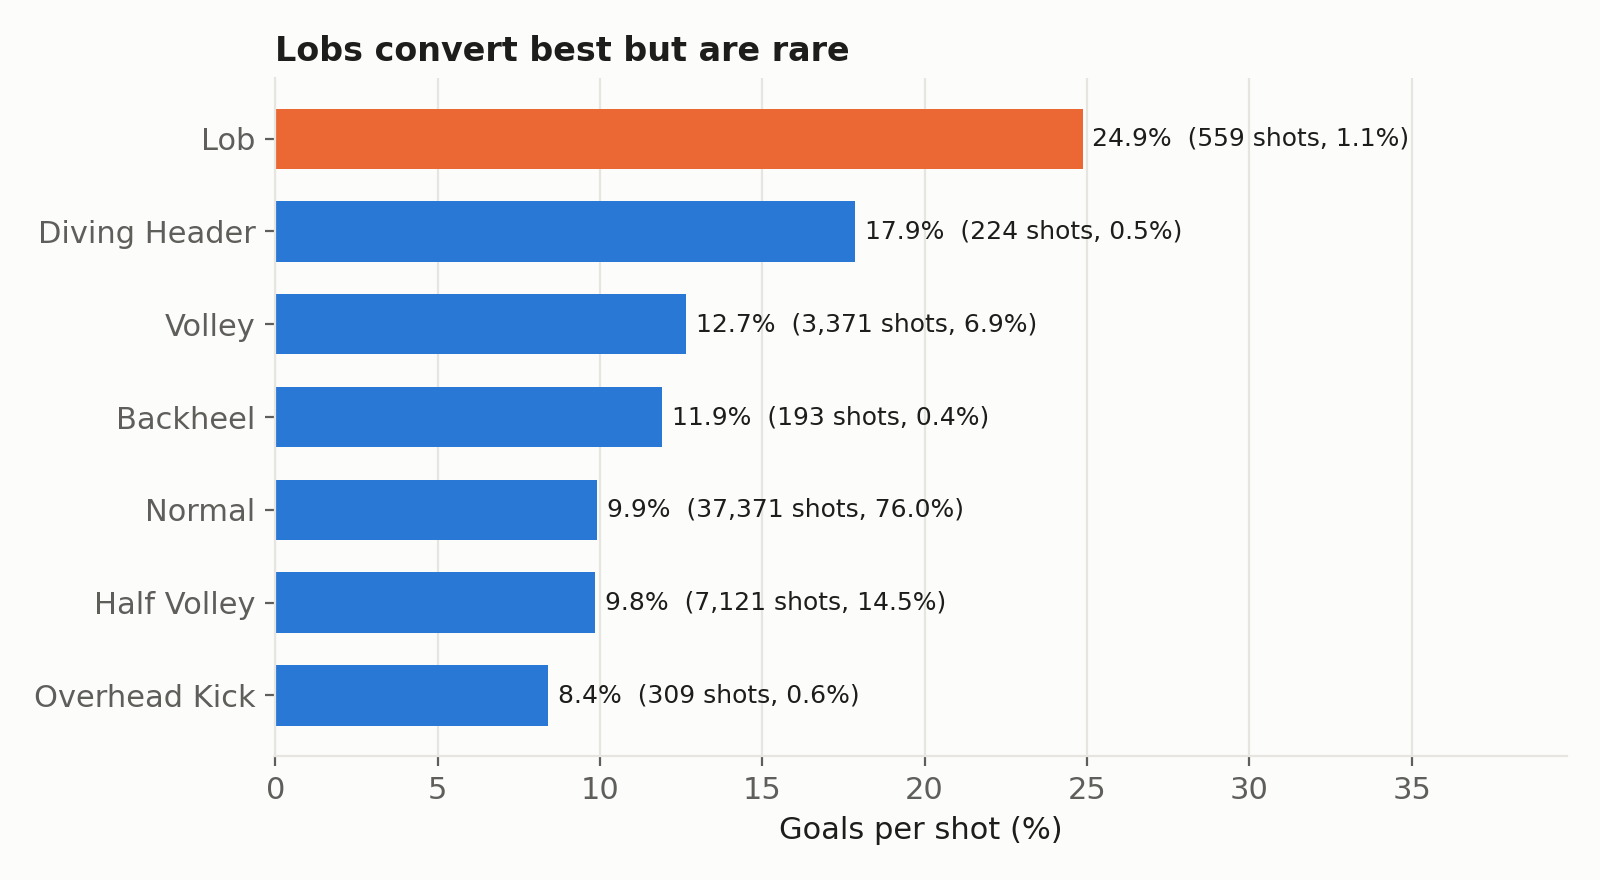
\includegraphics[width=0.9\textwidth]{images/tech.png}
    \caption{Goal Percentage by Shot Technique}
    \label{tech}
\end{figure}

Figure \ref{tech} shows that the lob had the highest conversion: 24.9\% of lobbed shots were goals, about one in four. Lobs are attempted only in particular situations, such as when the goalkeeper has come off the line, and they made up only 1.1\% of the open-play shots. Normal strikes were 76\% of shots and converted at 9.9\%.

With this, the Exploratory Data Analysis was concluded.

\newpage

\section{Feature Engineering}\label{feature}

Feature Engineering is the process of building new features from the existing data to improve predictive modelling. The features below were engineered from the raw shot data and the freeze frames. Section \ref{EDA} covered how each of them relates to goals.

\begin{itemize}
    \item Number of opponents in 5 yards: the number of opponents within 5 yards of the shooter
    \item Players between goal: the number of opponents, including the goalkeeper, inside the triangle formed by the ball and the two goal posts
    \item Shot Distance: the distance from the ball to the centre of the goal
    \item Goalkeeper Distance: the distance from the goalkeeper to the centre of the goal
    \item Shot Angle: the angle at the ball between the lines to the two goal posts
    \item Goal: the target, 1 for a goal and 0 otherwise
\end{itemize}

Each of these features can be seen in figure \ref{example}.

\newpage

\subsection{Mathematical Concepts Used}

As highlighted in \cite{maor2019pythagorean}, the distance formula gives the distance between any two points:

\begin{equation}
d = \sqrt{(x_2-x_1)^2 + (y_2-y_1)^2}
\label{distance}
\end{equation}

where $x_1, y_1$ and $x_2, y_2$ are the coordinates of the two points. The shot distance, for example, is the distance from the shot location to the centre of the goal at $(120, 40)$.

To calculate the Shot Angle, the Law of Cosines \cite{heath1956thirteen} was applied to the triangle formed by the ball and the two posts:

\begin{equation}
    c^2 = a^2 + b^2 - 2ab\cos\theta
    \label{law}
\end{equation}

where $a$ and $b$ are the distances from the ball to each goal post, $c$ is the distance between the posts (8 yards), and $\theta$ is the shot angle. An example can be seen in figure \ref{example}, where the red lines are $a$ and $b$. Rearranged, equation \ref{law} gives the shot angle:

\begin{equation}
\theta = \arccos\left(\frac{a^2 + b^2 - c^2}{2ab}\right)
\end{equation}

\begin{figure}[!h]
    \centering
    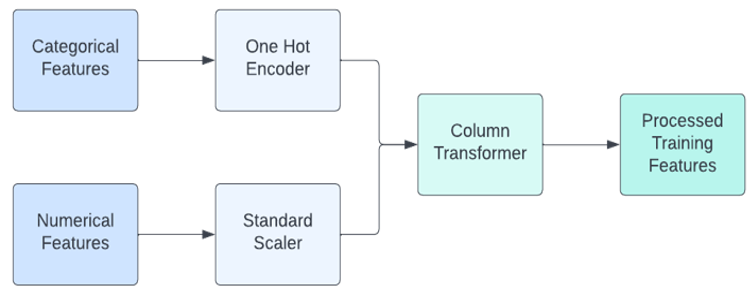
\includegraphics[scale=0.7]{images/featurepipe.png}
    \caption{Feature Processing}
    \label{featurepipe}
\end{figure}

\subsection{Final Features}

The model uses 13 features, the same as in the original edition:
\begin{itemize}
    \item 4 categorical features: body part (foot or head), pass type (ground, low, high or none), play pattern (regular or non-regular play) and first time (yes or no)
    \item 9 numerical features: shot distance, shot angle, opponents within 5 yards, players between the ball and goal, the x and y coordinates of the shot, goalkeeper distance, and the x and y coordinates of the goalkeeper
\end{itemize}

The two kinds of feature need different treatment before Machine Learning. Categorical features were one-hot encoded and numerical features were standardised, using the One Hot Encoder, Standard Scaler and Column Transformer of the Scikit-Learn library \cite{scikit-learn} (figure \ref{featurepipe}). After encoding, the 13 features become 19 model inputs. The encoder ignores categories it has not seen in training, so a rare category in new data cannot break the model.

\newpage

\section{Model Tuning and Evaluation}\label{test}

\subsection{Algorithms}

Four algorithms were used to predict xG:

\begin{itemize}
    \item Logistic Regression
    \item XGBoost
    \item LightGBM
    \item CatBoost
\end{itemize}

\subsubsection{Logistic Regression}
Logistic Regression is widely used for classification and predictive analytics. Based on a set of independent variables, it estimates the probability of an event, such as a goal. The log of the odds (the probability of success divided by the probability of failure) is modelled as a linear function of the features, so the output always lies between 0 and 1 \cite{1194264}.

\subsubsection{LightGBM}
LightGBM is a gradient boosting toolkit using tree-based learning, developed by Microsoft \cite{ke2017lightgbm}. It is designed to be fast and efficient:

\begin{itemize}
    \item Fast training and low memory use.
    \item Support for parallel, distributed and GPU learning.
    \item Able to handle large amounts of data.
\end{itemize}

\subsubsection{XGBoost}
XGBoost is a distributed gradient boosting library designed to be efficient, flexible and portable. It builds an ensemble of decision trees, each correcting the errors of the previous ones, and provides parallel tree boosting for a wide range of problems \cite{Chen:2016:XST:2939672.2939785}.

\subsubsection{CatBoost}
CatBoost is a gradient boosting library developed by Yandex. It builds symmetric trees and uses ordered boosting, which reduces overfitting, and it handles categorical data well \cite{DBLP:journals/corr/DorogushGGKPV17}.

\subsection{Splitting the Data by Match}

Shots from the same match are not independent: they share the same teams, the same conditions and often the same passage of play. If shots from one match are in both the training and the test set, the test result is too optimistic. The data was therefore split by \textbf{match}: 20\% of the matches (524 matches, 12,009 shots) were held out as the test set, and the models were trained on the other 2,092 matches (48,994 shots). No match has shots on both sides. The original edition split individual shots at random, so its test set shared matches with its training set.

\subsection{Hyper-Parameter Tuning}

Hyper-parameter tuning searches for the settings that make a model perform best \cite{hyperparameter}. Each model's settings were chosen with Randomized Search with cross-validation (RandomizedSearchCV in Scikit-Learn \cite{scikit-learn}) on the training matches only:
\begin{itemize}
    \item 5-fold cross-validation, with the folds also grouped by match
    \item 20 settings tried for Logistic Regression, XGBoost and LightGBM, and 12 for CatBoost, which is slower to train
    \item settings scored by \textbf{log loss}, because xG must be a good probability, not only a good ranking of shots
\end{itemize}

The settings searched were:
\begin{itemize}
    \item Logistic Regression: the regularisation strength $C$
    \item Tree models: the depth of the trees (or number of leaves), the number of trees, the learning rate, the L2 regularisation, and for XGBoost and LightGBM the share of rows and columns used for each tree and the minimum size of a leaf
\end{itemize}

The model with the best cross-validated log loss was chosen as the final model before the test set was used. The test set was used once, to report the results in chapter \ref{results}.

\subsection{Evaluation Metrics}

An xG value is a probability, and xG totals are used to judge players and teams. A good xG model must therefore not only rank shots well; its probabilities must also match how often goals are actually scored. Each model was evaluated on:
\begin{itemize}
    \item \textbf{Log loss}: how close the predicted probabilities are to the outcomes (1 for a goal, 0 otherwise). Lower is better. It punishes confident wrong predictions heavily, and it is the main measure used in this study. For reference, always predicting the average goal rate of 10.3\% gives a log loss of about 0.33.
    \item \textbf{Brier score}: the mean squared difference between the predicted probability and the outcome. Lower is better.
    \item \textbf{AUC}: the area under the ROC curve, the probability that a randomly chosen goal gets a higher xG than a randomly chosen miss. Higher is better; 0.5 is guessing. AUC measures ranking only, so a model can have a good AUC and still predict far too many or too few goals.
    \item \textbf{Calibration error (ECE)}: the shots are split into 10 equal-size groups by predicted xG, and in each group the mean xG is compared with the actual share of goals. ECE is the average gap, weighted by group size. Lower is better.
    \item \textbf{Predicted ÷ actual goals}: the total xG divided by the number of goals. 1.00 is perfect; above 1 means the model predicts too many goals.
\end{itemize}

StatsBomb's own xG, available for every shot, was evaluated on the same shots as a reference point.

\subsection{Out-of-Fold xG for Team and Player Analysis}

To analyse teams and players (section \ref{res:teams}), every shot needs an xG from a model that has not seen it. The final model was therefore also trained 5 times, each time on 80\% of the matches, and used to predict the other 20\%. Every one of the 61,003 shots gets an xG from a model that never saw its match. These \textit{out-of-fold} predictions are used for all team and player tables.
